%Linea Para poder completar automaticamente las citas con el Sublime
%No hace el documento, se puede borrar esta linea si no se usa el Sublime
%------------------------------------------------------------------------------
 \newcommand{\NoBiblioMeso}[1]{
 \ifthenelse{\equal{#1}{verdadero}}{}{\bibliography{Referencias/base_bibliografica}}
 \NoBiblioMeso{verdadero}}
 %-----------------------------------------------------------------------------

%Formato (Nombre de capitulo largo o corto), nombre del capitulo, resumen y estilo de la
%Portada del Capitulo
%------------------------------------------------------------------------------
 
 %Formato en si, titulo en dos renglones
 \FormatoCapituloDosLineas
 
 %Nombre y etiquete para referir
 \chapter{Métodos novedosos de síntesis de películas delgadas mesoporosas}
 \label{chap:Mesoporosos}

 %Para que no salga el numero de pagina en la portada del capitulo
 \thispagestyle{empty}
	
 %Resumen del Capitulo en Italica
 \noindent\textit{En este capítulo se exponen los resultados obtenidos para la fabricación y caracterización de películas delgadas mesoporosas. Se desarrollan metodologías y tratamientos alternativos a la calcinación, con el objetivo de obtener \pdm\space a menores temperaturas, y así compatibilizar con sustratos lábiles, poliméricos y con técnicas empleadas en microelectrónica. Se evaluó la estabilidad de las películas, adherencia a los electrodos, porosidad, accesibilidad, diámetro de poros, cuellos, control del espesor y demás variables que se consideraron relevantes para su aplicación como película permeoselectiva para iones en sensores electroquímicos}
 
 %Indice de capitulo alineada al borde inferior de la pagina, nueva pagina
 \vfill
 \minitoc
 \newpage
 %-------------------------------------------------------------------------------

\section{Introducción}

	Existen una gran variedad de precursores para controlar la composición y la estructura de películas delgadas mesoporosas de óxidos (PDM). Estas se pueden conformar tanto de óxidos puros, como SiO$_2$, TiO$_2$, ZrO$_2$ o de óxidos de mixtos de metales como (Si,Zr)O$_2$ o (Si,Ti)O$_2$; en general de óxidos metálicos de formula (M,M')O$_2$ siendo M y M', Si, Ti, Zr, Ce o Hf por enumerar los más utilizados.

	También existe una gran variedad de agentes moldeante para establecer el tamaño y la estructura espacial de los poros (F127, P123, Brij58, CTAB, etc) \cite{angelome2011,schuth2013,Soler-Illia2006,Soler-Illia2002a}. Este trabajo se centró exclusivamente en la síntesis de \pdm\space basadas en óxido de silicio para generar la estructura inorgánica. En la mayoría de los casos se utilizó puro, y en algunos combinado con óxido de circonio (ZrO$_2$). Para controlar el tamaño y estructura espacial de los poros se utilizó el copolímero de bloque Pluronic F127, bromuro de hexadeciltrimetilamonio (CTAB) y polioxietileno[20] cetil éter (Brij58). Esta elección no fue arbitraria, sino que se hizo en base a premisas bien fundamentadas:
		
		\begin{enumerate}

		\item El SiO$_2$ es procesable por técnicas sol-gel a través de diferentes precursores, es económico y fundamentalmente es el óxido mas utilizado en microelectrónica, aspecto fundamental en este trabajo para compatibilizar los procesos \textit{top-down} y \textit{bottom-up}.

		\item Tiene una química rica, bien conocida, forma enlaces covalentes con el carbono y es fácilmente funcionalizable pos-síntesis mediante el agregado de una gran variedad de grupos funcionales orgánicos o biológicos. Esta característica resulta fundamental para conferir selectividad de los sensores.

		\item No presenta absorción en el UV/Vis, esta propiedad es fundamental para poder, eventualmente lleva a cabo reacciones de polimerización dentro de los nanoporos, sin tener interferencias por absorción de luz.

		\item Como agente moldeante se utilizó F127, CTAB y Brij58 de forma de obtener \pdm\space con tamaño de poros bien variados, con diámetros que van desde los 10 a los \SI{2}{\nm}.

		\end{enumerate}
	
	Una vez elegidos los componentes esenciales que darán estructura a la película activa, se hizo foco en variar los sustratos. Ya que, al ser el objetivo final de la tesis sentar las bases para la fabricación de sensores multiselectivos, se debían explorar las distintos soportes para las películas mesoporosas, de forma de poder abarcar un rango amplio de materiales para distintos usos.

	Se depositaron los soles base sílice sobre silicio monocristalino, vidrio y películas delgadas de Au, con el objetivo de estudiar el comportamiento en cada uno de estos sustratos. Para poder comparar los resultados con la bibliografía\cite{Soler-Illia2006,Brinker1990} se decidió, en una primera etapa, tratar las películas por la ruta clásica de calcinación, explicada en la sección \ref{sec:cond_y_extr}, pág. \pageref{sec:cond_y_extr}. Impuestas estas condiciones de temperatura, se eligieron sustratos térmicamente estables:

		\begin{itemize}

			\item \textit{Portaobjetos de vidrio}. Se utilizó para todo tipo de experimentos exploratorios, por ejemplo para pruebas de depósito, cortes o diseños, ya que es el más económico del que disponemos, de superficie plana y con la misma composición que el sol, lo cual minimiza el estrés térmico entre el sustrato y la película.

			\item \textit{Silicio monocristalino, orientación cristalina [100]}. Las películas depositadas sobre silicio se utilizaron para obtener resultados de espectroscopía de absorbancia IR, para hacer elipsoporosimetrías e imágenes MEB principalmente. El silicio ofrece también un mayor contraste para visualizar las \pdm\space que el vidrio o el oro, por lo que se usó también para estimar la uniformidad de espesor sin la necesidad de utilizar microscopio, evaluando la homogeneidad a la largo de la superficie a través del color del depósito, el cual resulta de la interferencia óptica.
		
			\item \textit{Películas delgadas de Au}. El Au es el material elegido para los electrodos de los sensores. Sobre ellos se llevaron a cabo las pruebas electroquímicas, se evaluaron fenómenos de transporte, accesibilidad y propiedades de permeoselectividad. También se utilizó para obtener imágenes de MEB. 

			\end{itemize}
	
	En una segunda etapa, una vez dominada la química y física para obtener soles estables, películas homogéneas de espesor controlado y poder depositar sobre una amplia variedad de sustratos térmicamente estables, se dedicará el resto del capitulo a la discusión sobre métodos pos-depósito. Dicho tratamientos tienen por objetivo preservar la estructura del cristal líquido y extraer el molde sin necesidad de recurrir a procesos de calcinación ($\text{T} \geq 350^\circ \text{C}$).

	El desarrollo de métodos alternativos a la calcinación para condensar y extraer el molde supramolecular tienen varios própositos y surge de necesidades concretas. Por un lado, disminuir la temperatura permite compatibilizar los procesos \textit{bottom-up} (utilizados en la síntesis de las \pdm), y los procesos \textit{top-down} (necesarios para fabricar los sensores). Por otro lado, permite incluir sustratos no aptos para altas temperaturas (orgánicos en su mayoría) y de esta forma diversificar las opciones a la hora de elegir soportes para fabricar sensores basados en \pdm.\cite{Doshi2000a,Wagner2013,Innocenzi2013,Soler-Illia2002a,Zhang2005}.

	La gran mayoría de los autores emplean temperaturas típicamente entre \SI{350}{\celsius} y \SI{600}{\celsius} para producir materiales mesoporosos en general.\cite{Kresge1992,Beck1992,DiRenzo1997}  Dicho rango de temperatura tiene como ventaja que promueve la condensación del óxido y, a su vez, calcina el surfactante (materia orgánica) dando lugar a la formación de los poros. Sin embargo, para obtener un control adecuado sobre la estructura final, antes de la calcinación se debe estabilizar el arreglo micelar, es decir la estructura que actúa de molde supramolecular. Es abundante en la literatura los trabajos que se concentran en optimizar condiciones experimentales para estabilizar diferentes organizaciones espaciales de poros, empleando diferentes precursores con diversos surfactante\cite{Huo1996,Herregods2013,Grosso2001}. Existen muchos tratamientos y estrategias de síntesis para lograr dicho control basados en pH o variaciones del mismo durante la síntesis\cite{Doshi2000a,Soler-Illia2011,Boissiere2000,Huo1996,GonzalezSolveyra2017,Ichinose2002}, ciclos de P$_\text{H$_2$O}$\cite{Cagnol2002,Soler-Illia2012}, tiempos de envejecimiento\cite{Malfatti2009,Grosso2001} y rampas de temperatura\cite{Huang2002,Andrini2016,Soler-Illia2006,Rohlfing2005} por citar algunas de las variables mas influyentes. En general todas estas etapas pre-calcinación de los citados trabajos son a temperaturas moderadas, alrededor de los \SI{100}{\celsius} y destacan la importancia de controlar estás variables y, en el mejor de los casos, poder mantener la integridad estructural de la fase inorgánica luego de la calcinación. 

	Las publicaciones en las cuales se reporten métodos alternativos a la calcinación para la extracción del molde supramolecular son escasas. En el año 2000 Clark y col.\cite{Clark2000} emplean UV ($\lambda=187-$\SI{254}{\nm}) para generar una atmósfera oxidante rica en O$_3$ de forma de remover el surfactante. El método lo aplican con éxito sobre películas de sílice estructuradas con Brij56, sin embargo el arreglo de poros muda de hexagonal a cúbica luego de la exposición al UV. Los trabajos de Huang y col. en 2002\cite{Huang2002} y Zhang y col. en 2005\cite{Zhang2005} utilizan plasma para remover el molde. El primero emplea plasma de oxígeno sobre \pdm\space de TiO$_2$ y el segundo adapta el método para utilizarlo sobre mesoporosos en base sílice con plasma de argón. Ambos trabajos llegan a la conclusión de que la estructura se desordena, cambia el grado de porosidad y el control sobre la estructura final es poco predecible. Horiuchi y col.\cite{Horiuchi2011} en 2011 propone un proceso fotocatalítico para remover el surfactante. Para ello modifican la superficie de las \pdm\space de sílice con TiO$_2$, irradian con UV (con lámpara de HgXe) y concluyen que el TiO$_2$ interviene activamente en la oxidación y remoción del Brij78, el cuál fue utilizado como molde. Utilizaron \pdm\space de sílice sin modificar como experimento control y bajo estas condiciones no observaron evidencia de que el surfactante abandone la película.

	Los métodos citados en el párrafo anterior como alternativa a la calcinación, parecen promisorios. Sin embargo presenta algunas dificultades en su aplicación. El uso de plasma es aparentemente difícil de controlar y la penetración en las \pdm\space es poca. El uso de UV requiere de surfactantes fotodegradable o bien asistir la oxidación del molde con alguna modificación fotoactiva.

	En este trabajo se optó, como alternativa a la calcinación y a los métodos mencionados, extraer el surfactante por inmersión en solvente. Existen antecedentes de trabajos en los cuales se realiza este tipo extracción empleando como solvente etanol acidificado a una temperatura de \SI{200}{\celsius} \cite{Angelome2008,Calvo20210,Calvo2010,Fuertes2009}. Esta temperatura fue elegida por los autores para promover la condensación de la fase inorgánica sin comprometer la integridad de las funciones orgánicas incorporas en las películas. Para avanzar aún más en esa dirección, en este trabajo, se exploró una gama de procesos y condiciones de contorno para condensar la pared inorgánica y extraer el molde orgánico de películas delgadas mesoporosas de SiO$_2$ reduciendo todavía más la temperatura, por debajo de los \SI{130}{\celsius}.

	La búsqueda de procesos de síntesis con temperaturas de condensación extracción suaves permite fabricar los electrodos sobre Au metalúrgico o carbono (ver capitulo \ref{chap:Microfabricacion}, donde se desarrolla en profundidad estos aspectos) e incorporar sustratos poliméricos, como acrílico, resinas de poliéster, polibutileno de tereftalato (PBT), polietileno de tereftalato (PET), abriendo la posibilidad de utilizar una gama de materiales mucho mas amplia y abaratando costos. Veremos que mediante los procedimientos desarrollados es posible extender considerablemente el uso de sustratos para depositar \pdm\space en base sílice, abarcando virtualmente a cualquier superficie de baja rugosidad cuyo material sea estable por encima de los \SI{130}{\celsius}, incluyendo materiales flexibles.
	
\section{Síntesis de películas delgadas mesoporosas}
		
		Para la síntesis de las películas mesoporosas se utilizaron modificaciones de los procesos conocidos como <<Autoensamblado inducido por evaporación>> desarrolladas por el grupo de Brinker.\cite{Brinker1999} En el capitulo \ref{chap:Introduccion}, pág. \pageref{sec:mesoporosos}, se hizo breve introducción sobre los aspectos teóricos de este proceso y en el capitulo \ref{chap:Materiales}, pág. \pageref{sec:sintesis_mesoporosos}, se detallan los aspectos experimentales para la obtención de las \pdm. Se recuerda la nomenclatura usada en el capítulo \ref{chap:Materiales}; \pdmF\space y \pdmC\space para películas delgadas mesoporosas de SiO$_2$ estructuradas con Pluronic F127 y CTAB respectivamente; \pdmZ\space y \pdmZB\space para películas delgadas mesoporosas mixtas SiO$_2$/ZrO$_2$ estructuradas con F127 y Brij58 respectivamente.

		En los apartados que siguen se discuten los resultados obtenidos durante la fabricación de las \pdm\space por el método tradicional de depósito seguido de calcinación. Se discuten detalladamente los aspectos para controlar la homogeneidad, adherencia al sustrato, espesor y porosidad. Ésta será la base de conocimientos fundamentales para extrapolar y usar en el desarrollo de métodos de síntesis alternativos a la calcinación tratados en el resto del capítulo.

	\subsection{Control de la homogeneidad y espesor}
		
		Las técnicas más utilizadas para el depósito de películas por sol-gel son \textit{dip-coating} y \textit{spin-coating}. 
		Pensando en establecer las bases para la fabricación de sensores, se eligió trabajar exclusivamente por \textit{spin coating} con la intención de, en un futuro, escalar la síntesis, ya que esta técnica de síntesis permite obtener recubrimientos homogéneos en superficies extensas, en una sola cara y sobre sustratos con una gran variedad de texturas. De hecho es la que se utiliza en la megaindustria de los semiconductores.\cite{Franssila2004,Jaeger2001} 

		

			\begin{figure}[hb!]
	 	   	    \begin{subfigure}[t]{0.325\textwidth}
		        	\includegraphics[width=0.95\textwidth]{Imagenes/CTAB-Si.jpg}
		       		\caption{\pdmC\space sobre una oblea de silicio.}
		         	\label{fig:F127_vidrio}
		     		\end{subfigure}
	     		\begin{subfigure}[t]{0.325\textwidth}
		        	\includegraphics[width=0.95\textwidth]{Imagenes/CTAB-Au.jpg}
		       		\caption{\pdmC\space sobre un electrodo de Cr\textbar Au.}
		         	\label{fig:F127_silicio}
		     		\end{subfigure}
	     		\begin{subfigure}[t]{0.325\textwidth}
		        	\includegraphics[width=0.90\textwidth]{Imagenes/CTAB-electrodo.jpg}
		       		\caption{\pdmC\space sobre un arreglo de electrodos (diseño 1).}
		         	\label{fig:F127_Au}
		     		\end{subfigure}
	 	   	    \begin{subfigure}[t]{0.325\textwidth}
		        	\includegraphics[width=0.95\textwidth]{Imagenes/F127-Si.jpg}
		       		\caption{\pdmF\space sobre una oblea de silicio.}
		         	\label{fig:CTAB_vidrio}
		     		\end{subfigure}
	     		\begin{subfigure}[t]{0.325\textwidth}
		        	\includegraphics[width=0.95\textwidth]{Imagenes/F127-Au.jpg}
		       		\caption{\pdmF\space sobre un electrodo de Cr\textbar Au.}
		         	\label{fig:CTAB_silicio}
		     		\end{subfigure}
	     		\begin{subfigure}[t]{0.325\textwidth}
		        	\includegraphics[width=0.95\textwidth]{Imagenes/F127-electrodo.jpg}
		       		\caption{\pdmF\space sobre un arreglo de electrodos (diseño 2).}
		         	\label{fig:CTAB_Au}
		     		\end{subfigure}
	     		\caption[Películas mesoporosas sobre distintos soportes.]{Fotografías de las \pdm\space obtenidas por \textit{spin-coating }sobre distintos sustratos para los dos surfactantes utilizados: F127 y CTAB.}
	     		\label{fig:fotos_films}
	     	   	\end{figure}

		 Primero se establecieron las rampas de aceleración y velocidad final del \textit{spinner}; los tiempos de estabilización en cámara de humedad; los tiempos de calentamiento y calcinación, de forma de obtener películas homogéneas, sin fisuras y del espesor deseado. Los detalles del proceso se encuentran en la sección \ref{sec:deposito_pdm} y \ref{sec:cond_y_extr}, pág. \pageref{sec:deposito_pdm}. 

	     En la figura \ref{fig:fotos_films} se muestran fotografías de las \pdm\space obtenidas para los surfactante utilizados y los distintos sustratos. 


		 Allí se pueden destacar dos características de las \pdm: 1) la continuidad, ya que no se ven ni grietas ni fisuras y, 2) la homogeneidad en el color de interferencias. Dicho color es indicador de que el espesor es constante en toda la superficie, salvo en los bordes debido, precisamente, a los efectos de borde generados por la rotación del \textit{spinner}\cite{Franssila2004,Jaeger2001}.

		 La ausencia de discontinuidades microscópicas (grietas o fisuras) se pudo corroborar con imágenes MEB, donde se ve que el depósito es homogéneo en la superficie (ver figura \ref{fig:sem_homogeneidad}). En dichas imágenes también se observan detalles del arreglo poroso, y, en el caso del F127 se ve que dicho arreglo poroso esta homogéneamente distribuido también a lo largo del eje transversal a la superficie, como se muestra en la ampliación de la figura \ref{fig:sem_homogeneidad2}.
		

				\begin{figure}[bh!]
		 	   	    \begin{subfigure}[t]{0.495\textwidth}
			        	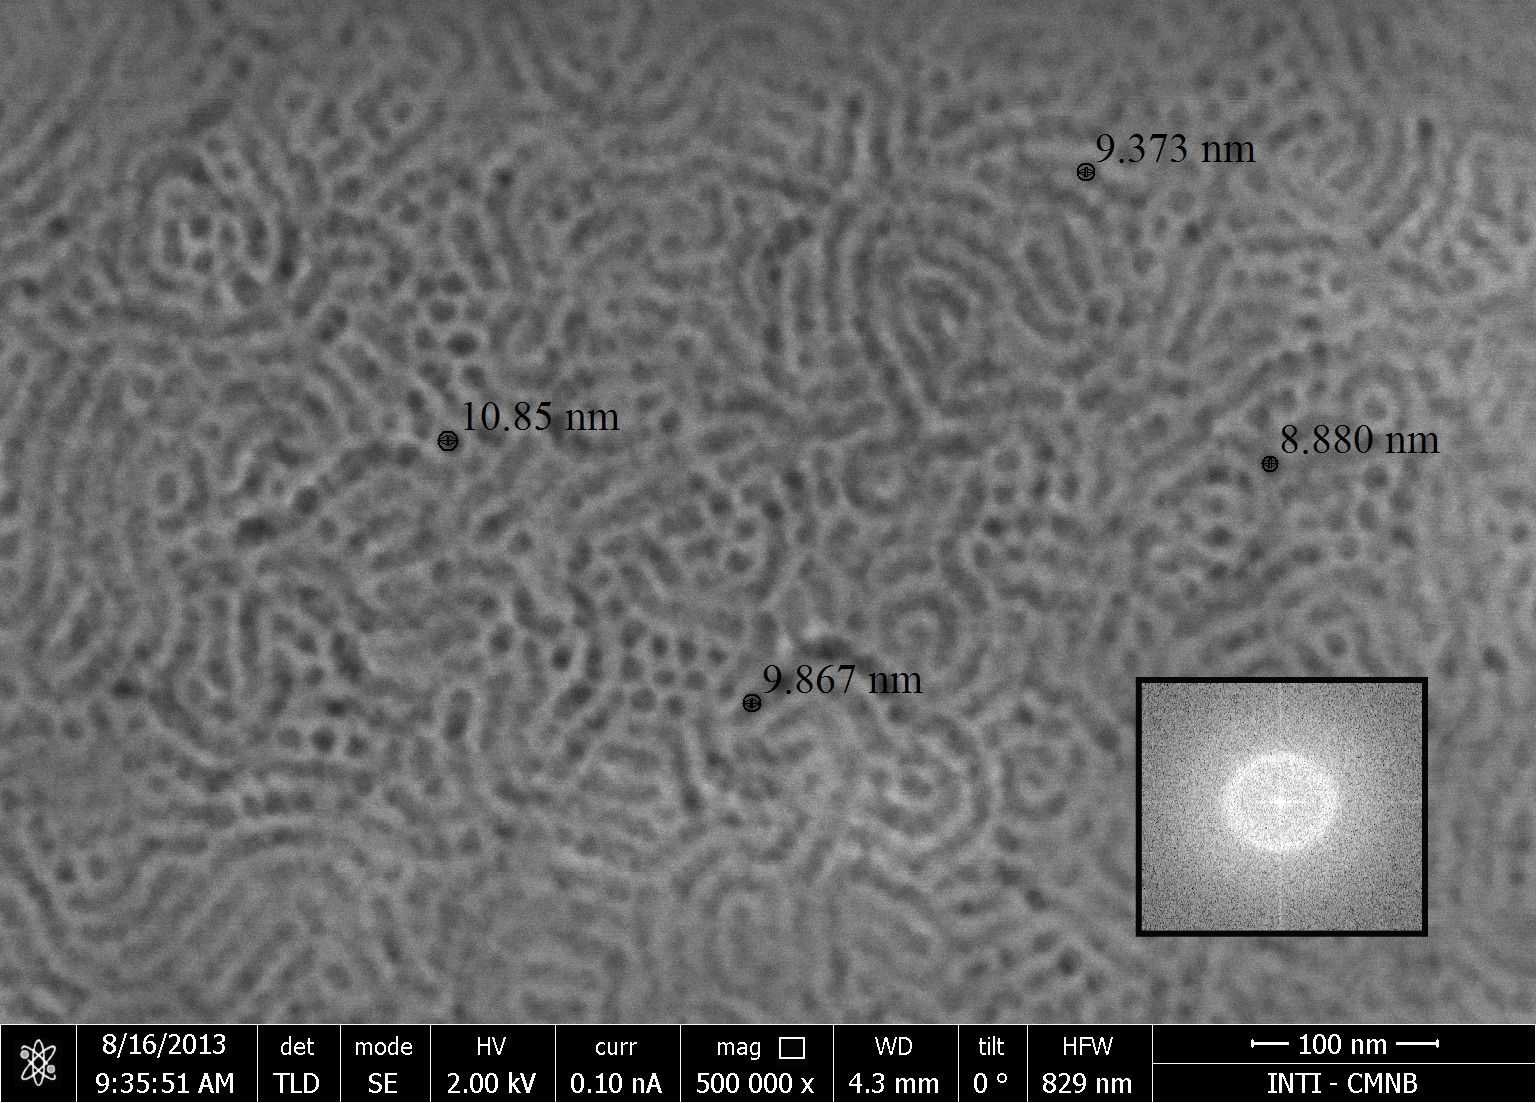
\includegraphics[width=\textwidth]{Imagenes/Superficie-F127-medidas.jpg}
			       		\caption{Microscopía electrónica donde se observa la superficie de una \pdmF\space con poros de \SI{10}{nm} de diámetro en promedio. Recuadro: FFT de la imagen completa.}
			       		\label{fig:sem_homogeneidad1}
			       		\end{subfigure}
			       	\begin{subfigure}[t]{0.495\textwidth}
			 	   	    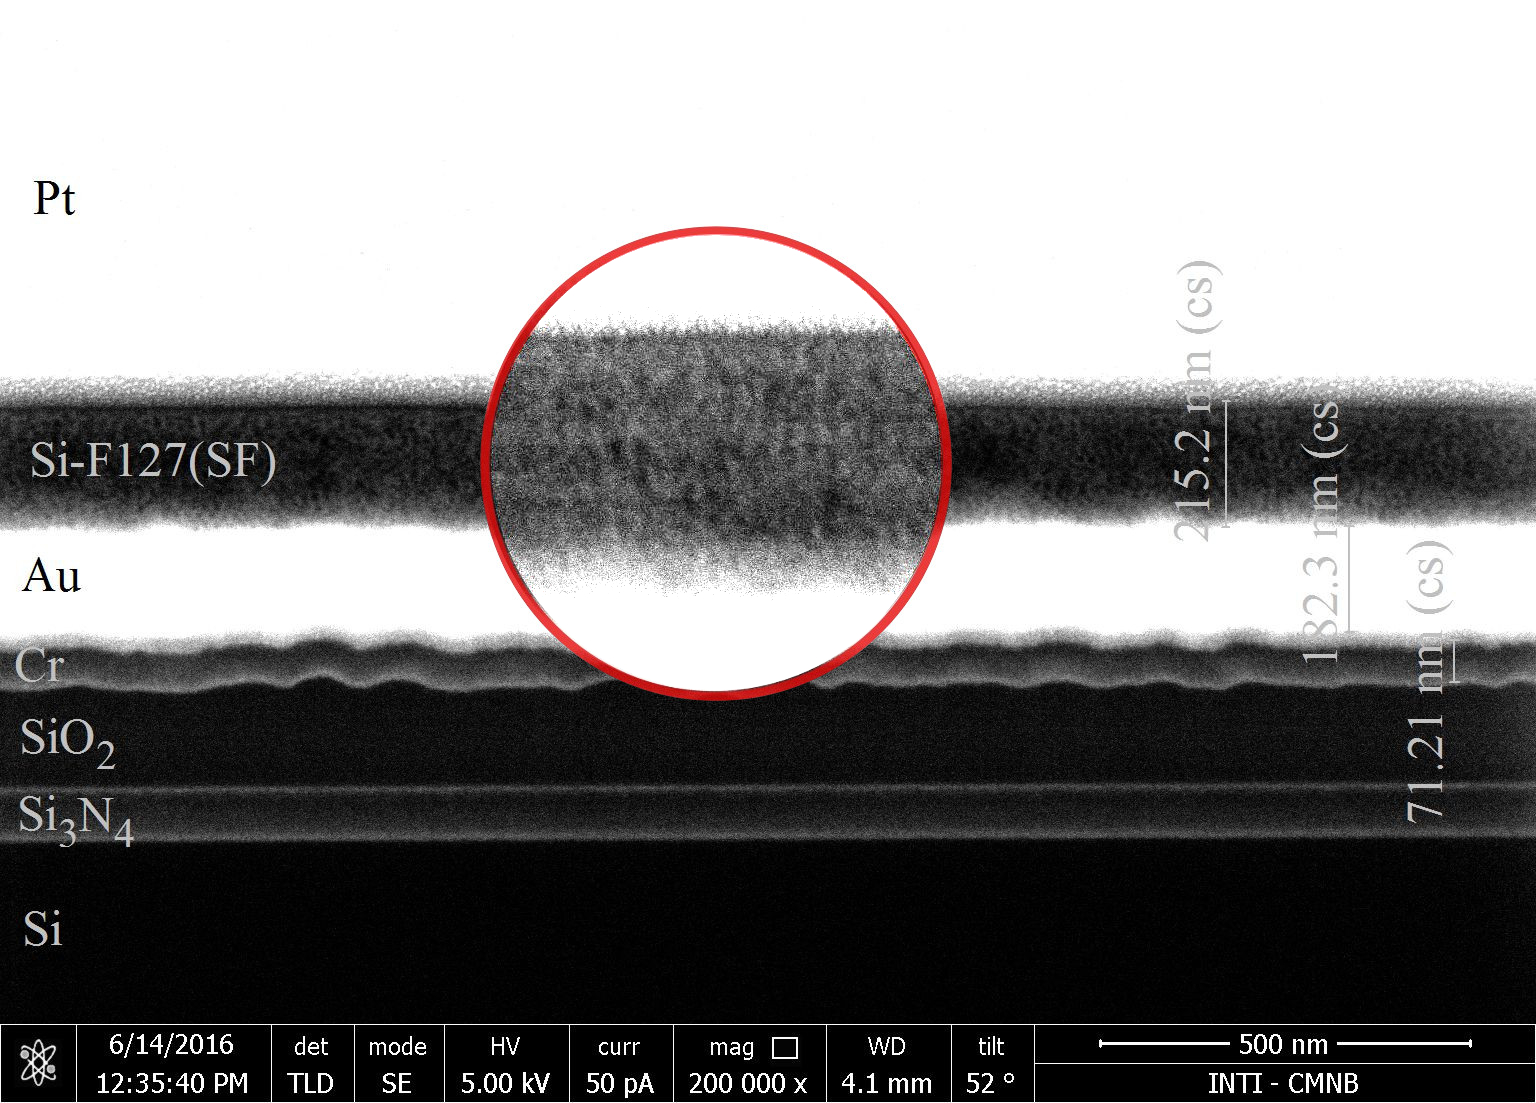
\includegraphics[width=\textwidth]{Imagenes/Perfil-F127.jpg}
			       		\caption{Corte transversal por FIB de una \pdmF\space desde se puede medir el espesor y observar los nanoporos a lo largo del eje transversal de la película.}
			       		\label{fig:sem_homogeneidad2}
			       		\end{subfigure}	
			       	\begin{subfigure}[t]{0.495\textwidth}
			        	\includegraphics[width=\textwidth]{Imagenes/Superficie-CTAB-medidas.jpg}
			       		\caption{Microscopía electrónica donde se observa la superficie regular de muestra \pdmC\space con poros de \SI{3}{nm} de diámetro en promedio.}
			       		\label{fig:sem_homogeneidad3}
			       		\end{subfigure}
					\begin{subfigure}[t]{0.49\textwidth}
			 	   	    \includegraphics[width=\textwidth]{Imagenes/Perfil-CTAB.jpg}
			       		\caption{Corte transversal por FIB de una muestra \pdmC\space en la cual se puede medir el espesor de la película. La resolución transcersal de la técnica no es suficiente para observar los nanoporos.}
			       		\label{fig:sem_homogeneidad4}
			       		\end{subfigure}	
					
					\vspace{-2mm}
					 \caption[MEB \pdmC\space y \pdmF.]{Microscopia para sistemas de sílice porosos con CTAB y F127 calcinados sobre silicio con electrodos de Cr\textbar Au (a y c). Secciones transversales pot microscipía FIB donde se puede apreciar la homogeneidad en el espesor de las películas (b y d).}
					 \label{fig:sem_homogeneidad}	
				     \vspace*{0.2cm}
				     \end{figure}
 	
		 El espesor se controla variando las condiciones de aceleración y velocidad final del \textit{spin-coater}, por lo tanto, para cada condición, se obtiene un espesor diferente. Las rampas de aceleración que se han utilizado para las \pdm\space se muestran en la figura \ref{fig:spin}. Tener control y conocimiento del espesor de las películas es importante para calcular o estimar otras magnitudes, por ejemplo concentración dentro de los poros o la distancia características de difusión. 

		 Algunos autores han desarrollado un marco teórico para establecer la dependencia del espesor con la velocidad de rotación en depósitos de películas poliméricas, encontrando una relación matemática según: \cite{Norrman2005,Meyerhofer1978,Bornside1989,Lora1990}
	
			\begin{equation}
			  t = k_1 \omega^{\alpha}
			  \label{eq:spin_meso}
			  \end{equation}		
	
		donde $k_1$ y $\alpha$ son constantes empíricas que dependen de la concentración del monómero, del solvente, del sustrato, de la interacción sol/sustrato y  de las propiedades reológicas del sol. Tal como se mostró en la ecuación \ref{eq:spin_meso}, y siguiendo los reportes de la literatura, el valor de $\alpha$ parece mantenerse contante y en las cercanías de $\alpha=-0.5$para una gran cantidad de polímeros. 

		Para controlar el espesor de los depósitos se realizaron mediciones del mismo en función de la velocidad final de rotación.  Dichas mediciones fueron tomadas en todos los casos por elipsoporosimetría ambiental (EPA) y sólo en algunos casos selecionados se contrastaron por MEB/FIB, obteniéndose valores comparables por ambas metodologías. Una vez establecido un valor de rotación de referencia se midieron en forma sistemática para cada tratamientos pos-depósito, con ambos surfactantes. Los valores de dichas mediciones se encuentras resumidos en la tabla \ref{tabla:resultados}.
		Los gráficos de la figura \ref{fig:esp} corresponden a la mediciones de espesores en sistemas calcinados. Fueron ajustados matemáticamente por la ecuación \ref{eq:spin_meso} y se obtuvieron valores de $k_1=6413\pm 2300$ y $\alpha=-0.44 \pm 0.04$ para \pdmF\space y $k_1=7601\pm 1800$ y $\alpha=-0.44 \pm 0.04$ para \pdmC. Dichos resultados siguen la tendencia esperada; disminución del espesor con el aumento de la velocidad angular y decaimiento exponencial con $\alpha \approx -0.5$. 

		
			\begin{figure}[!ht]
				\begin{subfigure}[t]{0.495\textwidth}
				\includegraphics[width=\textwidth]{Graficos/Esp_F127.pdf}
				\end{subfigure}
				\begin{subfigure}[t]{0.495\textwidth}
				\includegraphics[width=\textwidth]{Graficos/Esp_CTAB.pdf}
				\end{subfigure}
				\caption[Espesor en función de la velocidad angular]{Control del espesor en función de la velocidad de velocidades angulares para valores comprendidos entre 1000 y \SI{4000}{\minute^{-1}} en sistemas calcinados estructurados con F127 (izquierda) y CTAB (derecha). Todas las mediciones fueron llevadas a cabo por EPA.}
				\label{fig:esp}		
				\end{figure}
	
	\subsection{Adherencia al sustrato de las \pdm}	

		 En numerosos trabajos se ha demostrado la producción de películas delgadas mesoporososas de sílice (con surfactantes como F127, P123, CTAB, Brij56, Brij58, etc.) sobre sustratos de vidrio o silicio. En ninguno de ellos se menciona la existencia de problemas de adherencia al sustrato \cite{Angelome2008,Fuertes2010,Violi2015}. Resulta natural utilizar sustratos de silicio o vidrio debido a la compatibilidad estructural y química que comparten con las películas en base sílice. De hecho tanto película como sustrato son óxidos de silicio. Se conoce que luego de tratamientos térmicos para condensar y calcinar el surfactante, las películas sufren una contracción uniaxial a lo largo del eje normal a la superficie del sustrato debido a la fuerte adherencia al sustrato.\cite{Grosso2004,Soler-Illia2012,Chougnet2005} Uno de los pilares de este trabajo es el depósito de \pdm\space en base silicio sobre sustratos metálicos, más precisamente sobre Au. Sin embargo, se sabe desde hace décadas, que los metales nobles no tienen una buena adherencia sobre sustratos no-metálicos\cite{Kern1990,Hieber1976}, con lo cual es de esperar que también se experimenten problemas de adherencia al querer depositar un sol sobre una película delgada de Au. \cite{Meyer2004,Nugen2009,nasa1973} En las próximas secciones se exponen los resultados que ponen de manifiesto estos problemas y se proponen algunas solución para mejorar la adherencia de las \pdm\space sobre electrodos de Au.

		\subsubsection{Adherencia de \pdm\space sobre electrodos de Au}

			\subsubsection*{\pdm\space estructuradas con F127}

			En los electrodos en los cuales se depositó \pdm\space estructuradas con Pluronic F127 sobre películas de Au, se observó, en algunos casos, adherencia deficiente. 
			
			Las voltametrías cíclicas (VC) del gráfico \ref{fig:adherencia_F127} corresponden a respuesta de la sonda \aminorutenio (la cual difunde a través de la película) luego de 38 ciclos consecutivos, cantidad de ciclos suficiente para adsorber y saturar la \pdm\space con la sonda. Los mecanismos de transporte, adsorción y forma de las VC (tanto los cambios en la intensidad como los corrimientos en el potencial) se discuten en profundidad en el capitulo \ref{chap:Electroquimica}. 
			
				\begin{figure}[bh!]
				 	   	    \begin{center} 
				        	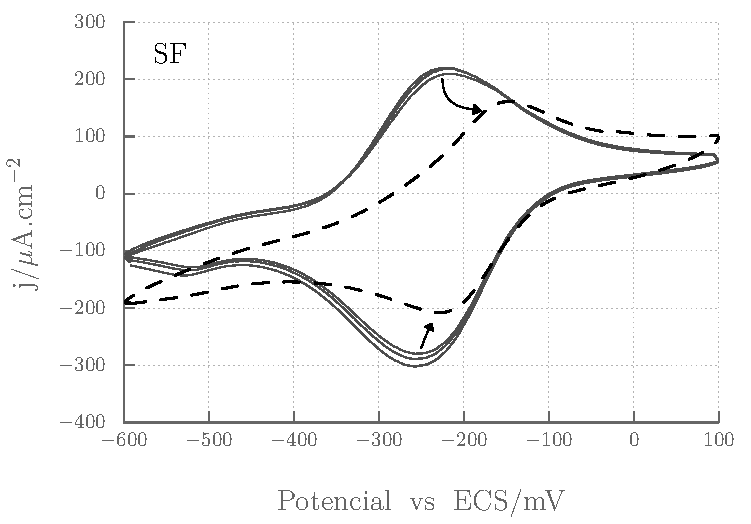
\includegraphics[width=0.70\textwidth]{Graficos/Adherencia_F127.pdf}
				       		\caption[Adherencia de \pdmF \space sobre una película delgada de Au.]{Serie de voltametrías cíclicas consecutivas, del ciclo 39 al 42, donde se evidencia la falta de adherencia de \pdmF\space sobre electrodo de Au. Las flechas negras indican un cambio repentino en el comportamiento, de un electrodo recubierto con una \pdm\space a un electrodo desnudo (curva punteada). Las VC fueron tomadas a \SI{50}{\milli\volt.\second^{-1}} usando de referencia ESC y con sonda \ru\space \SI{1}{\milli\Molar}.}
				         	\label{fig:adherencia_F127}
				     		\end{center}
				     		\end{figure}

			La observación de interés para determinar la adherencia es el cambio repentino en dos VC consecutivas (del ciclo 41 al 42), tanto en el corrimiento de potencial como en la disminución de la intensidad, indicado en el gráfico \ref{fig:adherencia_F127} mediante sendas flechas. Este cambio sugiere que el sistema muda de la típica respuesta de una sonda que se adsorbe en una \pdm, a la respuesta habitual de un electrodo desnudo de Au en el ciclo 42, marcado con linea de puntos. Esta comportamiento sugiere que la película no sufrió una disolución lenta y paulatina, sino que se desprendió del electrodo, total o parcialmente, en algún momento de la medición.	     		

			\subsubsection*{\pdm\space estructuradas con CTAB}	     		
				     		
			En los casos en los cuales se utilizó CTAB como molde para los poros, el comportamiento es algo diferente. Se manifiestan problemas de adherencia en la mayoría de los tratamientos alternativos, así como en la calcinación. Las películas presentan grietas y fisuras, macro y microscópicas y se observan desprendimientos antes de poder someter los sensores a cualquier medición electroquímica, es decir, apenas terminada la síntesis. Sólo se rescataron algunos pocos casos exitosos de formación de \pdmC\space sobre oro por calcinación, y con una superficie lo suficientemente extensa para poder realizar dichas mediciones. Éstos sirvieron para hacer experimentos de EQ conceptuales sobre transporte en poros (consultar capitulo \ref{chap:Electroquimica}), pero en la generalidad de los casos se observa desprendimiento de la película tal como muestran las imágenes de la figura \ref{fig:CTAB_adherencia}.

	     
				\begin{figure}[bh!]
		 	   	    \begin{subfigure}[t]{0.49\textwidth}
			        	\includegraphics[width=\textwidth]{Imagenes/Au_FCCTAB_adherencia1.jpg}
			       		\end{subfigure}
					\begin{subfigure}[t]{0.49\textwidth}
			 	   	    \includegraphics[width=\textwidth]{Imagenes/Au_FCCTAB_adherencia2.jpg}
			       		\end{subfigure}
					 \caption[Adherencia de CTAB sobre electrodos.]{Microscopías electrónicas donde se muestra la falta de adherencia de \pdmC\space sobre una película delgada de Au. Obsérvese los círculos grises que corresponden, en realidad a burbujas separadas del sustrato. La imagen de la derecha muestra una porción de \pdmC\space despegada y elevada.}
					 \label{fig:CTAB_adherencia}	
				     \end{figure}
			
			Además de la ya mencionada falta de adherencia de los óxidos sobre películas de Au, este desprendimiento se debe, sobre todo, a la interacción CTAB-Au. Es numerosa la información que se encuentra en la literatura sobre la interacción superficial de CTAB sobre películas delgadas y/o nanopartículas de Au. La principal aplicación se basa en la adsorción y autoensamblado del CTAB para controlar el crecimiento y estabilización de nanopartículas de Au. \cite{Cheng2003,Smith2008,Meena2013,Wang2013,Hamon2009} Algunos autores lo utilizan por encima de la concentración micelar crítica (cmc)\cite{Lim2014}o combinado con otros reactivos para favorecer el crecimiento cristalino en alguna dirección preferencial\cite{Smith2009}. Los electrodos de Au, depositados por pulverización catódica, generan películas policristalinas sin favorecer ninguna dirección cristalina.\cite{Svorcik2010,Bechelany2010} Sobre esta superficie las moléculas de CTAB o las micelas se adsorben. Su distribución y densidad a largo de la superficie del electrodo parece depender de la concentración, la orientación cristalina del Au, el solvente y la rugosidad de la superficie\cite{Meena2013,Lim2014}. La adsorción del surfactante en la superficie del electrodo, sumada a la poca adherencia propia del SiO$_2$, son factores que van en demerito de la adherencia y consecuentemente de la formación de \pdmC\space sobre electrodos de Au. %Si bien, como veremos más adelante, se aplicaron los métodos alternativos de síntesis para películas estructuradas con CTAB, estos fueron caracterizados para \pdmC\space sobre silicio. 
			Como se explica más adelante (ver sección \ref{sec:trat-vacio}), para obtener \pdm\space de poros pequeños ($\leq$\SI{5}{\nm}) sobre electrodos con superficies suficientemente extensas y sin presencia de discontinuidades, se recurrió al uso de un surfactante no-iónico, el Brij58.
							
		\subsubsection{Estrategias para mejorar la adherencia}\label{sec:adherencia}

			 En función de los resultados expuestos en la sección anterior queda claro que la falta de adherencia de las \pdm\space sobre oro es crítica para la elaboración de los sensores. Por otra parte, al fabricar electrodos de Au con un diseño arbitrario, se suma la dificultad de obtener películas delgadas continuas y adherentes sobre un sistema con dos regiones distintas en su superficie, óxido y metal.
 
             Las estrategias empleadas para promover la adherencia en estos sistemas se basaron en dos conceptos:
				\begin{enumerate}

					\item Optimizar el diseño de forma de minimizar el área metálica de los electrodos, pistas y contactos, ampliando la región del óxido para favorecer la adhenrecia de las \pdm.

					\item Realizar modificaciones superficial en los electrodos, tendiendo puntos de anclaje entre el electrodo y el esqueleto inorgánico de las \pdm.

					\end{enumerate}
			
			 La primera estrategia utilizada para promover una mayor adherencia de las \pdm\space a los sensores, se basa en minimizar el área de contacto electrodo-mesoporoso. Las mayoría de los resultados discutidos en este capítulo fueron realizados en \pdm\space sobre electrodos plenos de Au. Sin embargo, los sensores comprenden un conjunto de electrodos o microelectrodos sobre un sustrato dieléctrico (p. ej. SiO$_2$ o vidrio). Eligiendo un diseño adecuado se puede minimizar el área de los electrodos metálicos. De ésta forma las \pdm\space quedan adheridas fuertemente a los sectores del óxido, donde no está el Au. El resultado final es una película bien adherida sobre una superficie mixta soporte/electrodos.  La figura \ref{fig:adherencia_microelectrodo} representa de manera esquemática esta situación.
			
				\begin{figure}[!ht]
					\begin{center}
					\includegraphics[width=0.80\textwidth]{Esquemas/adherencia_microelectrodo.pdf}
					\caption[Adherencia a los microelectrodos.]{Esquema de un corte transversal de los sensores donde se observan los microelectrodos y la \pdm\space depositada sobre ellos. Las flechas indican las zonas de baja y alta adherencia.}
					\label{fig:adherencia_microelectrodo}
					\end{center}
					\end{figure}
					
					
			 La segunda estrategia se basa en modificar los electrodos mediante una funcionalización superficial, la cual se llevó acabo siguiendo el procedimiento detallado en el capitulo \ref{chap:Materiales}, sección \ref{sec:silanizacion}. Se buscó una molécula compatible con el sistema utilizado, capaz de vincular la superficie del electrodo e integrarse al esqueleto de las \pdm. Se usó para este fin el 3-mercaptopropil trimetoxisilano (MPTMS), el cual es fácilmente de ligar covalentemente al Au por el tiol\cite{Gosser,Byun2013}, y por el otro tiene el silano el cual es perfectamente compatible con el precursor de Si(IV) utilizado\cite{Wu2014,Wu2013,Chen2011}. En la figura \ref{fig:mod_sup} se muestra la molécula en cuestión y un esquema de como queda anclado la \pdm, mediante el MPTMS, al electrodo.
		
			 Una vez realizada la modificación superficial, se llevaron a cabo mediciones EQ para evaluar si los voltagramas sufren distorsiones debido a la funcionalización. Se realizaron dos comparaciones con propósitos diferentes: 1) verificar que la señal sobre un electrodo desnudo no se vea afectada significativamente por la presencia de MPTMS ligado a la superficie del Au; y 2) demostrar que la funcionalización del Au mejora la adherencia cuando se depositan \pdm\space sobre esta superficie modificada.

			 \begin{figure}[!ht]
							\begin{center}
							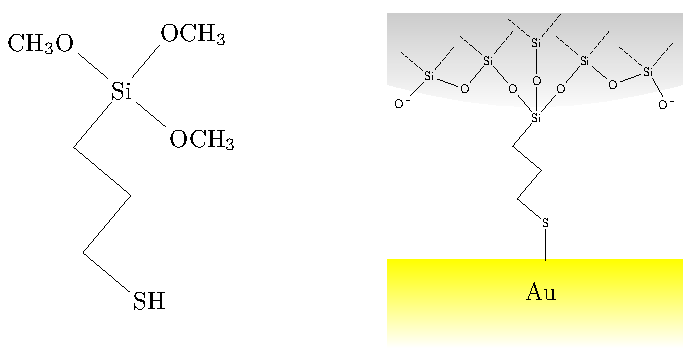
\includegraphics[width=0.70\textwidth]{Esquemas/mod_sup.pdf}
							\caption[Modificación superficial de los electrodos.]{Izquierda: Molécula de  3-mercaptopropil trimetoxisilano utilizada como ligante entre los electrodos y las \pdm. Derecha: Esquema pictórico de la modificación superficial con MPTMS.}
							\label{fig:mod_sup}
							\end{center}
							\end{figure}
										
			 En la figura \ref{fig:comparaciones_MPTMS-A} se presentan dos voltagramas en los cuales se compara la respuesta para \aminorutenio\space \SI{1}{\milli\Molar} con dos electrodos de Au, uno virgen y otro funcionalizado con MPTMS. Como se puede apreciar en el gráfico la respuesta es prácticamente igual para ambos tipos de electrodos, demostrando que la funcionalización con el tiol no modifica significativamente la respuesta electroquímica.

					\begin{figure}[!ht]
							\begin{center}
							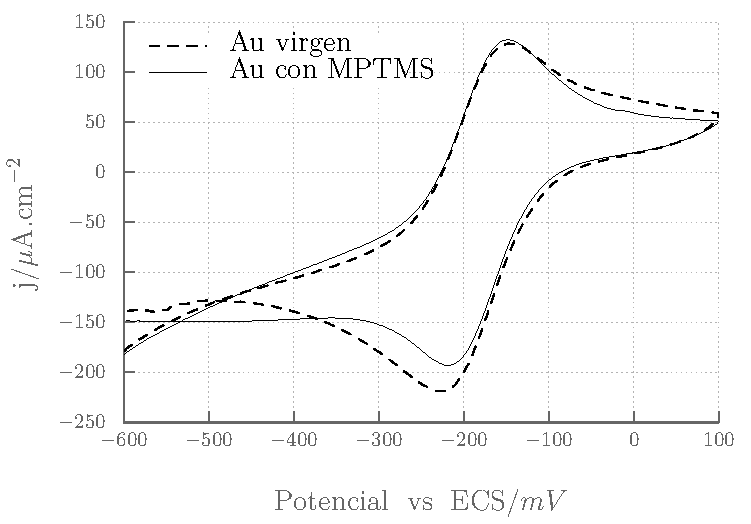
\includegraphics[width=0.70\textwidth]{Graficos/Comparacion_Au-MPTMS.pdf}
							\caption[Comparación de electrodos con y sin MPTMS]{VC para \aminorutenio\space \SI{1}{\milli\Molar} a \SI{50}{\milli\volt\per\second} sobre un electrodo virgen de Au (rojo) comparado con uno funcionalizado con MPTMS (negro). La funcionalización con el tiol no bloquea ni modificar el desempeño electroquímico de los electrodos.}
							\label{fig:comparaciones_MPTMS-A}
							\end{center}
							\end{figure}

             Las voltametrías cíclicas de la figura \ref{fig:comparaciones_MPTMS-B} muestran un típico experimento donde el \aminorutenio\space ingresa y a medida que va difundiendo a lo largo de una película \pdmF, se adsorbe sobre las paredes de la mismas. Dicho voltagrama esta constituido por 30 voltametrías cíclicas consecutivas correspondiente a los ciclos 45 al 75. A partir del ciclo 65 se ve una disminución en la intensidad de pico, la cual es compatible con un fenómeno de disolución de la película y no a un evento de desprendimiento. Los fenómenos de ingreso, adsorción y disolución de las películas se discute en profundidad en el capitulo \ref{chap:Electroquimica}.
       	
					\begin{figure}[!ht]
							\begin{center}
				 	   	    \includegraphics[width=0.70\textwidth]{Graficos/Comparacion_F127-MPTMS.pdf}
				       		\caption[Comparación de superficies con y sin MPTMS.]{Voltametrías cíclicas consecutivas para \aminorutenio\space \SI{1}{\milli\Molar} a partir del ciclo número 44 realizados a \SI{50}{\milli\volt.\second^{-1}} sobre electrodos modificados con MPTMS. La respuesta es de características similares a la obtenida para este tipo de sistemas, donde se observa el ingreso de la sonda, la adsorción y la disminución de la intensidad debido a un fenómeno de disolución. No se observa indicio alguno de falta de adherencia.}
						 \label{fig:comparaciones_MPTMS-B}	
					    \end{center}
					    \end{figure}
		
			 Ambas estrategias ideadas para promover la adherencia fueron aplicadas tanto a películas donde se uso F127 o Brij58 como surfactante. Además son complementarias y compatibles. Esto quiere decir que se puede optimizar el diseño para minimizar la superficie de electrodos y, a su vez, es posible funcionalizar con MPTMS las regiones de los electrodos, generando puntos de vinculación entre el mesoporosos y el electrodo. La funcionalización se debe lleva a cabo luego de depositar el Au y antes de realizar el decapado de la fotorresina (consultar sección \ref{sec:fotolito}, pág. \pageref{sec:fotolito}) y no sobre los sensores terminados. De esta forma la modificación queda delimitada sólo a las regiones donde están los electrodos, evitando reacciones colaterales como la silanización del vidrio o silicio con el MPTMS por el extremo del silanol.

			 Es importante resaltar que en los casos que no se utilizó MPTMS, el desprendimiento o despegue de las \pdm\space se hizo evidente por microscopía óptica o durante las mediciones EQ en una fracción de las casos, en otros se observaron grietas, fisuras o discontinuidades en las películas. En contrapartida, en los electrodos que se funcionalizaron con MPTMS, el 100\% de los casos llevaron a la formación de películas continuas, sin grietas y con buena adherencia.

\section{Métodos alternativos de síntesis de \pdm}
	
	 En esta sección se da cuenta de los resultados obtenidos en la fabricación y caracterización de \pdm\space por métodos alternativos a la calcinación. Como ya se mencionó anteriormente, el desarrollo de estos métodos surgió de necesidades que emergieron durante el proceso de fabricación de los sensores. Entre las principales necesidades se cuentan: disminuir la diferencia de expansión térmica entre las películas delgadas mesoporosas y metálicas, minimizar procesos difusivos, ampliar sustancialmente la gama de sustratos, mejorar la adherencia y disminuir costos.

	 En este sentido, se idearon metodologías que permiten disminuir la temperatura de procesado hasta \SI{130}{\celsius}, sin perder grado de condensación y manteniendo las características espaciales de los poros. Al no calcinar, se agrega una etapa extra, la eliminación del surfactante. Presentamos a continuación una tabla con la nomenclatura y una breve reseña de los procesos que se exploraron y que fueron descriptos en detalle en la sección \ref{sec:cond_y_extr}.

	 Se exponen primero los resultados de las caracterizaciones de las \pdm\space obtenidas por calcinación. El propósito de ésto es tener datos de referencia para comparar con los métodos alternativos. Luego se discuten los resultados que se obtuvieron por cada uno de ellos, los cuales se resumen en la tabla \ref{tabla:resultados}. Finalmente, se expone una discusión global comparando cada una de las técnicas, para cada uno de los métodos. Para facilitar la lectura, la información detallada microscópica y espectroscópica de cada proceso se encuentra en el anexo C.
	 
	  	 \begin{table}[h!] 
		 	 \caption[Tratamientos alternativos de síntesis de \pdm]{Nomenclatura de los métodos alternativos de síntesis de \pdm.}
			 \begin{tabular}{>{\raggedright\arraybackslash}m{1.9cm}>{\centering\arraybackslash}m{1cm}>{\raggedright\arraybackslash}m{0.9cm}>{\raggedright\arraybackslash}m{6.62cm}} 
			 \toprule
				 Método   &  Nomenclatura$^*$&  & Descripción \\ \midrule
				 Calcinado & CalSC CalSF& &  Condensación \SI{130}{\celsius} \SI{1}{hora}\hspace{2cm} Extracción \SI{350}{\celsius} \SI{2}{hora}\hspace{2cm} \\ \midrule
				 Simplificado & SimSC SimSF& &  Condensación \SI{130}{\celsius} \SI{1}{hora}\hspace{2cm} Extracción IpOH / H$_2$O pH=2 \\ \midrule
				 Prolongado & ProSC ProSF& & Condensación \SI{130}{\celsius} \SI{7}{dias}\hspace{2cm} Extracción IpOH / H$_2$O pH=2 \\ \midrule				
				 Vacío & VacSC VacSF VacZSF VacZSB& &  Condensación \SI{130}{\celsius} \SI{7}{dias}, P=\SI{e-5}{\milli\bar}\hspace{2cm} Extracción IpOH / H$_2$O pH=2 \\ \midrule
				 Ácido & ÁciSC ÁciSF& &  Condensación en atmósfera de HCl\hspace{2cm} Extracción IpOH / H$_2$O pH=2 \\ \midrule
				 Alcalino & AlcSC AlcSF& & Condensación en atmósfera de NH$_3$\hspace{2cm} Extracción IpOH / H$_2$O pH=2 \\ 
				\bottomrule
				   \end{tabular}\vspace*{2pt}
		    	  	\footnotesize{$^*$SC=sílice/CTAB, SF=sílice/F127, ZSF=circonio-sílice/F127, ZSB=circonio-sílice/Brij58.}
				   	\label{tabla:tratamientos}
				   \end{table}
	
	 \pagebreak\subsection{Método de calcinación}
	 	
	 		El tratamientos de calcinación luego del depósito del sol es una ruta sintética clásica utilizada por muchos autores para la producción de películas delgadas mesoporosas de óxidos\cite{Soler-Illia2002a,Brinker1999,Soler-Illia2006,Grosso2004,Innocenzi2013,angelome2011}. Consiste en estabilizar las \pdm\space mediante un tratamiento a humedad y temperatura controladas, seguidas de calcinación a \SI{350}{\celsius} para eliminar el molde. Los detalles técnicos se pueden consultar en la sección \ref{sec:cond_y_extr}, pág. \pageref{sec:cond_y_extr}.

	 	  \subsubsection{Análisis de la porosidad}

		 Como veremos en adelante, la porosidad y accesibilidad son factores que determinan la cantidad de analito que se adsorbe o difunde a través de las \pdm, por este motivo resulta fundamental tener herramientas para cuantificar dichas magnitudes. 

		 Del estudio de las películas por MEB se puede obtener información muy valiosa como tamaño y distribución de los poros, así como estudios de la organización espacial de los mismos mediante transformadas de Fourier (FFT). En la figura \ref{fig:F127_Si_Au} se muestran imágenes de MEB para películas \pdmF sobre distintos sustratos, cada una con su respectiva transformadas. De éstas, se deduce que se trata de un arreglo de poros con orden local con tamaños próximos a los de \SI{10}{\nm} de diámetro, coincidiendo la con información existente en la literatura\cite{urade2005,angelome2011,lee2006} y con los datos obtenidos por EPA (ver más adelante y consultar la tabla \ref{tabla:resultados} para mas información).  

			\begin{figure}[th]
		 	   	    \begin{subfigure}[t]{0.49\textwidth}
			        	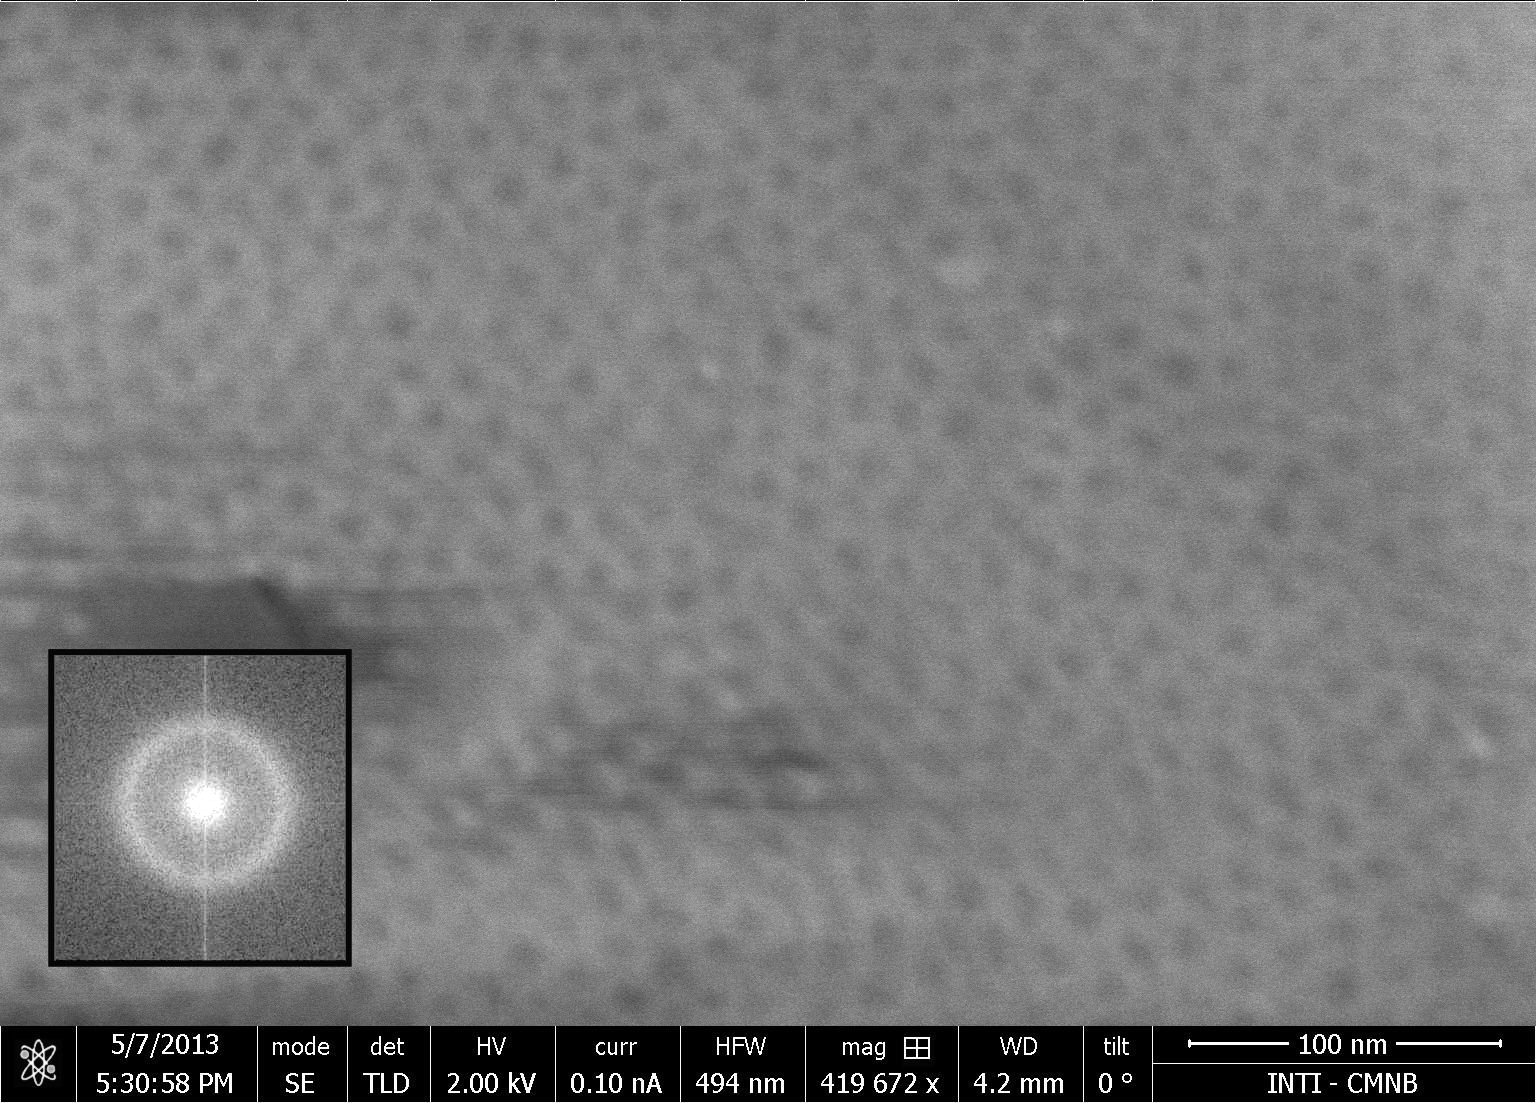
\includegraphics[width=\textwidth]{Imagenes/F127_Si_sup.jpg}
			       		\end{subfigure}
					\begin{subfigure}[t]{0.49\textwidth}
			 	   	    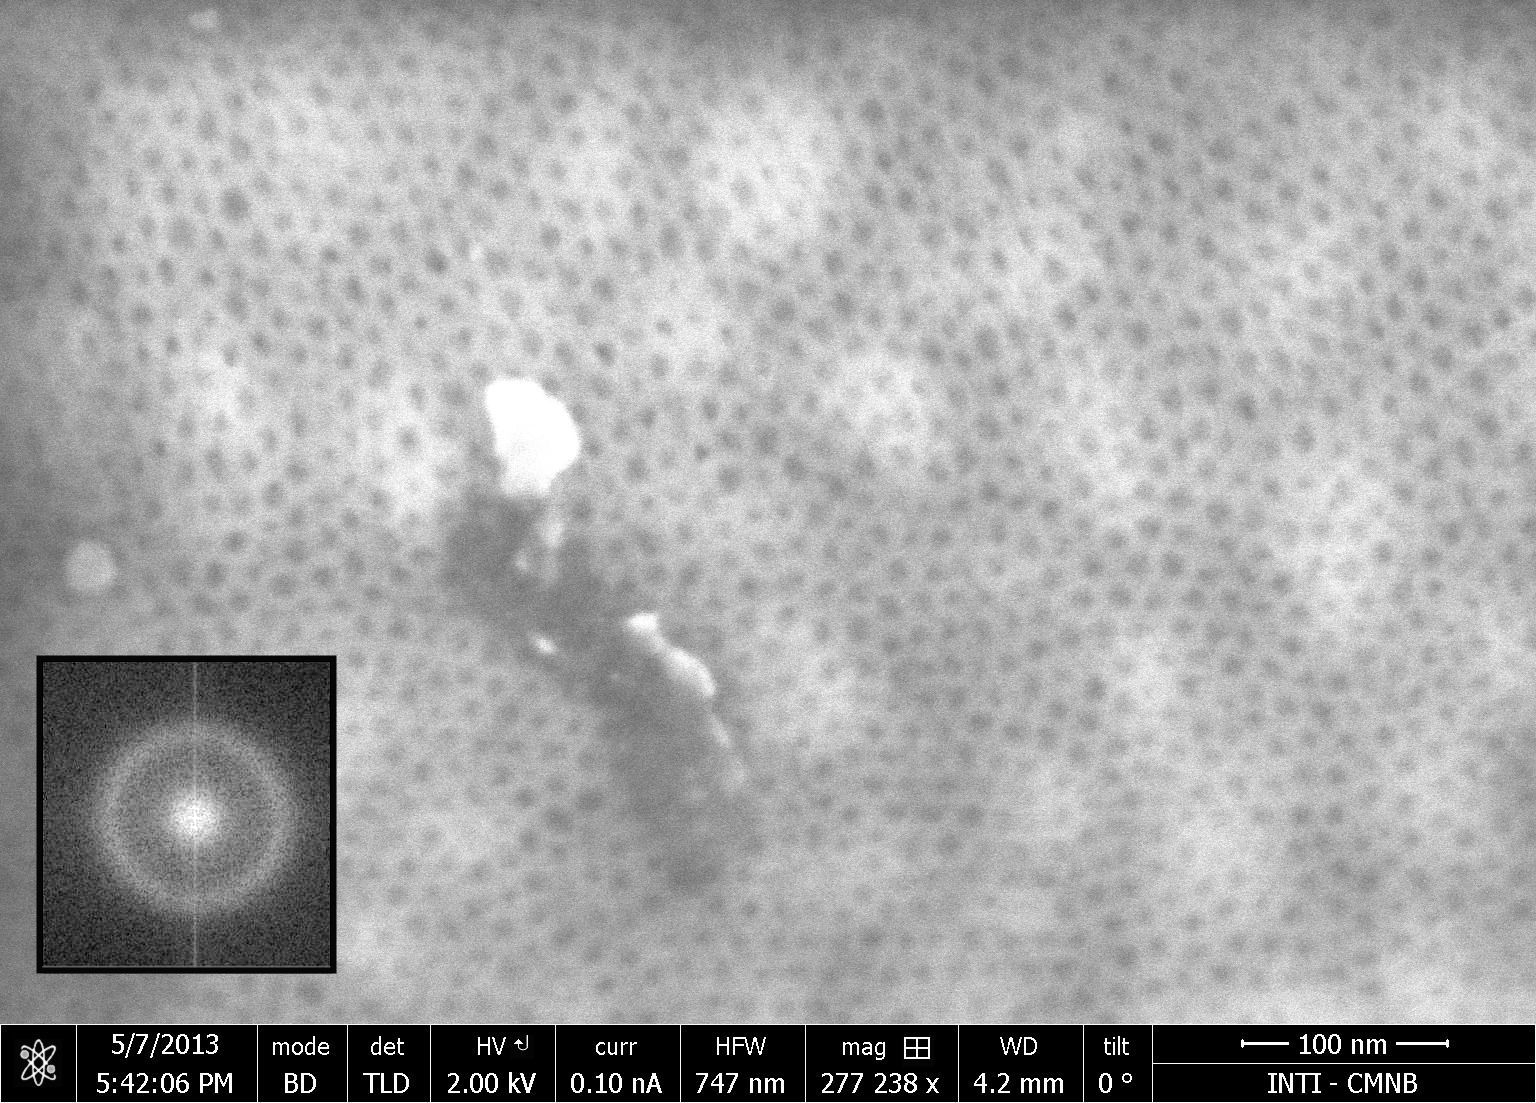
\includegraphics[width=\textwidth]{Imagenes/F127_Au_sup.jpg}
			       		\end{subfigure}
					\caption[MEB arreglo poroso para \pdmF\space sobre Si y Au.]{Microscopía electrónica de barrido de sistemas \pdmF\space y sus respectivas FFT. Se observa la distribución y homogeneidad de los poros en superficie. Izquierda: sobre sustrato de silicio. Derecha: sobre sustrato de Au.}	 
					 \label{fig:F127_Si_Au}
					 \end{figure}

		 En el caso de las películas porosas estructuradas con CTAB el análisis por MEB brinda una información más limitada, ya que el diámetro de los poros ($\approx$ \SI{3}{\nm}) esta en el límite de resolución de la técnica para muestras no conductoras. Sin embargo, alcanza para  ver que existe un sistema de poros (ver figura \ref{fig:sem_homogeneidad3}). En este caso, para hacer un estudio por imágenes mas completo, se debería recurrir a microscopía electrónica de transmisión (MET).

		 El estudio por MEB es sumamente útil en muchos aspectos; sin embargo, la información que brinda es de áreas muy pequeñas, superficial y no da información completa sobre la conectividad y cuellos de las películas. Es por ello que se recurrió a la técnica de elipsoporosimetría ambiental (EPA). Ésta es una técnica promedio, donde podemos obtener información valiosa sobre la accesibilidad de agua en los poros, se puede determinar el volumen poroso de las \pdm, la distribución de tamaños de poros y cuellos y la variación del espesor en función de la presión de vapor de agua relativa a la presión de saturación ($\text{P/P}_s$). Para valores crecientes de P/P$_s$, la adsorción en los mesoporos se produce a través de la formación de una monocapa y luego de multicapas de moléculas de agua sobre las paredes de los poros, seguida de condensación capilar, es decir, llenado de los poros con agua líquida. La posterior disminución de la presión externa resulta en la desorción mediante evaporación capilar, vaciando primero el centro de los poros, seguida por la desorción de la multicapa de solvente presente en las paredes de los mismos. Para cada punto de P/P$_s$ en equilibrio se tiene un valor del índice de refracción efectivo ($n$), de esta forma se construye la isoterma de adsorción/desorción de agua. Los cálculos realizados para obtener información estructural (volumen poroso, y distribución de poro y cuello) a partir de las isotermas se basaron en el protocolo detallado los trabajos del grupo de Sánchez y Baklanova\cite{Baklanov2000,Boissiere2005,Sakatani2006}. Los detalles experimentales de esta técnica se presentaron en el capitulo \ref{sec:elipso}, pág. \pageref{sec:elipso}.

		 En las figuras \ref{fig:F127_EPA} y \ref{fig:CTAB_EPA} se presentan las isotermas de adsorción de agua para sistemas calcinados \pdmF\space y \pdmC. Se observa que ambas son de tipo IV, según la clasificación de Brunauer\cite{Gregg1967,Violi2015,Fuertes2010}. Este tipo de isotermas con histéresis entre la rama de adsorción y la de desorción es característico de materiales con mesoporos, donde los poros se llenan por condensación capilar. Por otro lado el ciclo de histéresis se podría clasificar como un ciclo intermedio entre H1 y H2, según la clasificación IUPAC\cite{Thommes2015}. Esto es indicativo de una estructura de poros de tamaño uniforme que formar parte de un red compleja con efectivos significativos sobre la adsorción de solvente.\cite{Thommes2015,Gregg1967,Lowell2004,Sing1985}

		 En las figuras \ref{fig:F127_PSD} y \ref{fig:CTAB_PSD} se muestran las distribuciones de tamaño de poro para estos sistemas. Dichas distribuciones se obtuvieron a partir de las isotermas, y se extrajo información estructural tanto de la rama de adsorción como de la de desorción.


		     	  	\begin{figure}[!ht]
		     	  		\begin{subfigure}[t]{0.495\textwidth}
		     	  		\includegraphics[width=\textwidth]{Graficos/SI_F127_Calcinado_EPA.pdf}
						\caption{Elipsoporosimetría de una \pdmF\space depositada sobre silicio sintetizada por calcinación.}
						\label{fig:F127_EPA}
						\end{subfigure}
						\begin{subfigure}[t]{0.495\textwidth}
		     	  		\includegraphics[width=\textwidth]{Graficos/SI_F127_Calcinado_PSD.pdf}
						\caption{Distribución de tamaño de poro y cuello correspondientes a la isoterma de (a).}
						\label{fig:F127_PSD}
						\end{subfigure}
						\caption[Elipsoporosimetría para sistemas \pdmF.]{(a) Curva de adsorción/desorción de agua para una \pdmF\space. La misma corresponde a una isoterma de tipo IV con un lazo de histéresis de tipo H1/H2, lo cual se concuerda con materiales mesoporosos con poros y cuellos interconectados. (b) Distribución de poros y cuellos con tamaño de poros uniformes, de aproximadamente \SI{10}{\nm} de diámetro.}
						\end{figure}
					\begin{figure}[!ht]
		     	  		\begin{subfigure}[t]{0.495\textwidth}
		     	  		\includegraphics[width=\textwidth]{Graficos/SI_CTAB_Calcinado_EPA.pdf}
						\caption{Elipsoporosimetría de una \pdmF\space sobre sustrato de silicio sintetizada por el método clásico de calcinación.}
						\label{fig:CTAB_EPA}
						\end{subfigure}
						\begin{subfigure}[t]{0.495\textwidth}
		     	  		\includegraphics[width=\textwidth]{Graficos/SI_CTAB_Calcinado_PSD.pdf}
						\caption{Distribución de tamaño de poro y cuello correspondientes a la isoterma de (a).}
						\label{fig:CTAB_PSD}
						\end{subfigure}
						\caption[Elipsoporosimetría para sistemas \pdmC.]{(a) Curva de adsorción/desorción de agua para una \pdmC\space . La misma corresponde a una isoterma de tipo IV con un lazo de histéresis de tipo H1/H2, lo cual se concuerda con materiales mesoporosos con poros y cuellos interconectados. (b) Distribución de poros y cuellos con tamaño de poros uniformes, de aproximadamente \SI{3}{\nm} de diámetro.}
						\end{figure}	
		

		 	Del conjunto de resultados presentados cabe resaltar que son películas homogéneas, sin grietas ni discontinuidades tanto a nivel macro como microscópico, con poros organizados localmente y distribución de tamaños de poros y cuellos estrecha . Las \pdm\space estructuradas con F127 presentan poros y cuellos de 9 y \SI{4.5}{\nm} de diámetro respectivamente, mientras que las estructuradas con CTAB, 2.5 y \SI{2}{\nm}. También se pueden extraer los valores de $n$, porcentaje de volumen poroso (\%V) y espesor los cuales se resumen en la tabla \ref{tabla:resultados}. Estos valores son los que se usarán para establecer un parámetros de condensación y porosidad de las \pdm\space y se usaran como semilla para la discusión comparativa con los resultados obtenidos para el resto de los tratamientos.

	      \subsubsection{Análisis por FTIR}\label{sec:Analisis_IR}

		 Son muchos los trabajos en los cuales se caracterizan las películas delgadas de SiO$_2$ por IR\cite{Olsen1989,Almeida1990,Redol1997,Innocenzi2003}, y también muchos otros que recolectan y emplean dichos resultados.\cite{Angelome2008,Calvo2008,Calvo20210}.
		 El análisis de espectroscopia infrarroja por transformada de Fourier (FTIR) se utilizó en esta tesis para identificar y caracterizar la estructura inorgánica porosa de SiO$_2$, evaluar comparativamente la condensación del óxido, y determinar la presencia de grupos orgánicos, en particular residuos de surfactante. 

		 Innocenzi ha realizado un análisis completo y bien fundamentado sobre las vibraciones en el IR, de películas delgadas de SiO$_2$ tanto densas como mesoporososas.\cite{Innocenzi2003} Para los enlaces Si-O-Si, se observa la presencia de 4 modos de vibración óptico-trasversales (TO$_x$) y 4 modos óptico-longitudinales (LO$_x$) en películas delgadas de SiO$_2$. Aquellas películas de SiO$_2$ sintetizadas por sol-gel se caracterizan principalmente por presentar tres de los cuatro modos transversales, los cuales en general son tomados como huella digital para este tipo de materiales.\cite{Innocenzi2003,Angelome2008,Calvo2008} El modo TO$_1$, presenta una banda débil $\approx$\SI{460}{\cm^{-1}} asociada a movimientos de balanceo; el modo TO$_2$ está asociado a un estiramiento simétrico con un pico débil cercano a $\approx$\SI{800}{\cm^{-1}}; el modo TO$_3$ presenta un pico intenso centrado en $\approx$\SI{1075}{\cm^{-1}} y se asocia a vibraciones asimétricas del enlace Si-O-Si. 

		 		 \begin{figure}[!ht]
						\begin{center}
						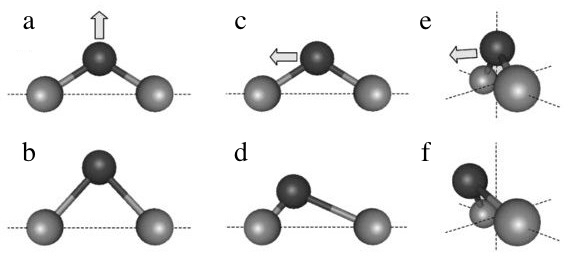
\includegraphics[width=0.90\textwidth]{Imagenes/modos-infra.jpg}
						\caption[Modos de vibración Si-O-Si]{Representación de los movimientos de vibración del oxigeno (gris oscuro) respecto de los átomos de silicio (gris claro).(a) y (b) estiramientos simétrico perpendicular a plano Si-Si. (c) y (d) estiramientos antisimétrico paralelo a la recta Si-Si. (e) y (f) balanceo perpendicular al plano Si-O-Si. La figura fue adaptada de la publicación \textit{Infrared spectrocopy of sol-gel derived silica-based films: a spectra-microstructure overvire}, J. Non. Cryst. Solids, 316(2-3), p. 309-319. }
						\label{fig:modos-ir}
						\end{center}
						\end{figure}

		 El modo TO$_4$ por lo general no es observable, algunos autores lo reportan como una banda muy débil en las cercanías de \SI{1150}{\cm^{-1}} \cite{Pai1986,Grosse1986}. La figura \ref{fig:modos-ir} es una representación esquemática de los tres principales modos de vibración: TO$_1$, TO$_2$ y TO$_3$.

		 En experimentos de incidencia normal a la superficie, solo deberían excitarse las vibraciones óptico-transversales, sin embargo se observan banda de vibraciones correspondientes a modos óptico-longitudinales asociadas a oscilaciones colectivas acopladas TO-LO\cite{Pai1986,Grosse1986,Innocenzi2003}. Los modos ópticos-longitudinales, LO$_1$ y LO$_2$ no son visibles, y LO$_3$, aparece como un hombro de la banda TO$_3$ a mayores frecuencias. La observación experimental de LO$_4$ es escasa, cuando se observa aparece como una banda muy débiles en la zona comprendida entre 1200 y \SI{1150}{\cm^{-1}} \cite{Pai1986,Grosse1986}.
		 
		  \begin{figure}[!th]
						\begin{center}
						\includegraphics[width=0.83\textwidth]{Graficos/IR_Denso.pdf}
						\caption[FTIR SiO$_2$ denso y SiO$_2$ mesoporoso.]{Espectro de absorción de IR de una película SiO$_2$ denso depositada por \textit{sputtering }comparada con una de SiO$_2$ mesoporoso. Se observa, para las \pdm, la aparición de un marcado hombro en \SI{1180}{\per\cm} debido al acoplamiento TO$_3$-LO$_3$ y un pico correspondiente a la vibración $\nu$Si-OH.}\index{sputtering@\textit{sputtering}}
						\label{fig:IR-denso}
						\end{center}
						\end{figure}

		 \pagebreak Otra observación relevante, realizadas por Almeida y Pantano\cite{Almeida1990}, es la naturaleza del hombro presente en $\approx$\SI{1180}{\cm^{-1}}, el cual se intensifica con el aumento de la porosidad de la película y lo asocia a un acoplamiento de los modos LO$_3$ y TO$_3$ con predominancia de carácter LO. Este fenómeno parece estar asociado a la dispersión de la radiación IR dentro de los poros y la consecuente activación del modo longitudinal.	
			
		 Se pudo corroborar dicha observación en los espectros de la figura \ref{fig:IR-denso}, donde se compara una \pdm\space con una película delgada de SiO$_2$ depositada por \textit{sputtering}.  Allí se ve el hombro bien acentuado para la \pdm\space y una banda en $\approx$\SI{965}{\cm^{-1}} asociada al estiramiento Si-OH/Si-O$^-$; mientras que para la película de SiO$_2$ denso depositada por \textit{sputtering} ($n\sim 1.5$ a $\lambda=$\SI{600}{\nm})\cite{Vergohl1999} se observa la ausencia del hombro, aparición de la incipiente banda de LO$_4$ y desaparece la banda del Si-OH/Si-O$^-$.

		 Además del análisis de la estructura inorgánica, se utilizó FTIR para evidenciar la presencia del surfactante usado de molde para los poros. Se centrará la atención en las bandas que corresponden a las vibraciones del enlace C-H, las cuales aparecen en la zona de 2950 a \SI{2850}{\cm^{-1}}. En la figuras \ref{fig:IR_F127_calciando} y \ref{fig:IR_CTAB_calcinado} se comparan \pdm\space calcinadas \SI{350}{\celsius} y sin calcinar para los surfactantes utilizados. Se ve como desaparecen las bandas correspondientes a al vibración C-H debido a la eliminación del surfactante. Se conserva la forma del hombro a $\approx$\SI{1180}{\cm^{-1}} indicador de una estructura porosa y se observa la banda en en $\approx$\SI{965}{\cm^{-1}} asociada al estiramiento Si-OH/Si-O$^-$, el cual según algunos autores sólo desaparece cuando las películas son sometidas a T$>$\SI{500}{\celsius} debido a la condensación de grupos silanol en la superficie.\cite{Innocenzi2003,Almeida1990,Bertoluzza1982}

				\begin{figure}[b!]
						\begin{center}
						\includegraphics[width=0.83\textwidth]{Graficos/IR_F127.pdf}
						\caption[FTIR para una \pdmF.]{Espectro de absorción para una \pdmF\space antes y después de calcinar, donde se puede apreciar la aparición de un pico fuerte el cual correspondiente al surfactante F127.}
						\label{fig:IR_F127_calciando}
						\end{center}
						\end{figure}
			 
		  Estos espectros IR, obtenidos para películas calcinadas, se utilizarán de referencia para comparar con los espectros IR de \pdm\space producidas por métodos alternativos a la calcinación. 

		  \pagebreak Por un lado, se evalúa la presencia de poros, indicado por la presencia del hombro LO$_3$-TO$_3$ y  por otro, el grado de condensación, siguiendo la relación de picos Si-O-Si/Si-OH. Por último, la técnica es utilizada para corroborar la eliminación del surfactante por ausencia de la banda $\approx$\SI{2900}{\per\cm} correspondiente a la vibración C-H.

		  		\begin{figure}[h!]
						\begin{center}
						\includegraphics[width=0.83\textwidth]{Graficos/IR_CTAB.pdf}
						\caption[FTIR para una \pdmC.]{Espectro de absorción para una \pdmC\space antes y después de calcinar, donde se puede apreciar la aparición de un pico fuerte el cual correspondiente al surfactante CTAB.}
						\label{fig:IR_CTAB_calcinado}
						\end{center}
						\end{figure}

		  En la tabla que sigue, se asignan las vibraciones observadas que servirán de referencia para el análisis de resultados de las próximas secciones.

		 	\begin{table}[hb!] 
		 	 \caption[Asignación de vibraciones en el IR]{Bandas y asignación de vibraciones en el IR frecuentemente observadas a lo largo de la tesis.}
			 \begin{tabular}{>{\raggedright\arraybackslash}m{2.6cm}>{\centering\arraybackslash}m{2.55cm}>{\raggedright\arraybackslash}m{5.7cm}} 
			 \toprule
				 Posición (\si{\per\cm})   &  Vibración &  Presente en \\ \midrule
				 3500-3000	& $\nu_\text{OH}$ & H$_2$O, 2-propanol \\ \midrule
				 2950-2850  & $\nu_\text{C-H}$ & Molde (CTAB, Pluronic F127) \\ \midrule
				 2450		& CO$_2$ & CO$_2$ ambiental \\ \midrule
				 2000-1200  & H$_2$O & Estructura fina del H$_2$O\hspace{2cm} H$_2$O adsorbida  \\ \midrule
				 1250		& $\nu_\text{Si-O-Si}$ & SiO$_2$ denso LO$_3$ \\ \midrule
				 1170		& $\nu_\text{Si-O-Si}$ & SiO$_2$ denso LO$_4$ \\ \midrule
				 1075		& $\nu_\text{Si-O-Si}$ & SiO$_2$ TO$_3$ \\ \midrule
				 1180 (hombro) & $\nu_\text{Si-O-Si}$ & SiO$_2$ poroso acoplamieno LO$_3$-TO$_3$ \\ \midrule
				 965 		& $\nu_\text{Si-OH}$ & SiO$_2$ parcialmente condensado silanoles superficiales\\ \midrule 
				 800		& $\nu_\text{Si-O-Si}$ & SiO$_2$ denso TO$_2$ \\
				 \bottomrule
				   \end{tabular}
				   	\label{tabla:ftir}
				   \end{table}

	      \subsubsection{Accesibilidad de las PDM}\label{sec:acc}

			Hasta ahora se han evaluado muchos de los aspectos fundamentales para poder pensar en utilizar las películas mesoporosas de óxido de silicio como componentes de sensores: estructura porosa, volumen poroso, compatibilidad de sustratos, técnicas de depósito, control del espesor, etc. 

			Sin embargo, se debe considerar un aspecto crítico para utilizar estas películas como parte de un sensor electroquímico. Se debe garantizar el libre acceso de los analitos a través de los nanoporos, de forma de poder difundir hasta la superficie del electrodo, para que tenga lugar allí, la reacción electroquímica.

			Para evaluar el transporte de especies a través de los materiales, se coloca una solución con una sonda electroquímica adecuada, en la celda de medición en contacto con el electrodo. La forma en que fueron tomadas las medidas se explica extensamente en la sección \ref{sec:medidas_eq}, pág \ref{sec:medidas_eq}. 

			La figura \ref{fig:accesibilidad} muestra dos voltametrías cíclicas, una para \pdmF\space y otra para \pdmC\space en presencia de \aminorutenio\space \SI{1}{\milli\Molar} en solución de KCl \SI{0.1}{\Molar}. En ambos voltagramas se registra una respuesta electroquímica, demostrando que la superficie del electrodo se encuentra accesible. Los resultados sugieren que existe un camino percolativo en las \pdm, tanto si se estructuran con F127 o con CTAB, que permite, o bien que la señal electroquímica se propague desde el seno de la solución hasta el electrodo (transporte de carga) o bien que el analito difunda desde la solución al electrodo (transporte de masa). Los diferentes mecanismos de trasporte involucrados en estos experimentos, son tema central de esta tesis y se discuten en detalle en el capitulo \ref{chap:Electroquimica}. De estos experimentos preliminares se puede concluir que la síntesis de \pdm\space sobre electrodos lleva a películas que, al menos en parte, son accesibles y permiten a una sonda EQ difundir hasta la superficie del electrodo.   

						\begin{figure}[th]
				 	   	    \begin{subfigure}[t]{0.495\textwidth}
				        	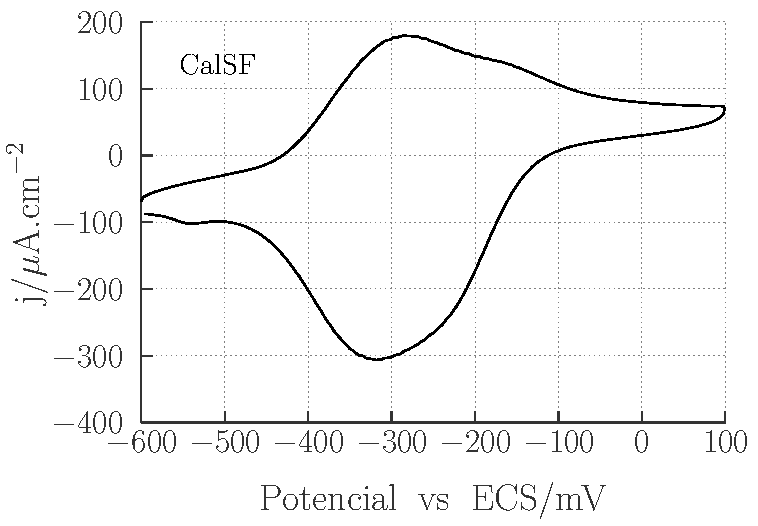
\includegraphics[width=\textwidth]{Graficos/SF-accesibilidad.pdf}
				       		\caption{Voltametría Cíclica sobre \pdmF}
				         	\end{subfigure}
				         	\begin{subfigure}[t]{0.495\textwidth}
				        	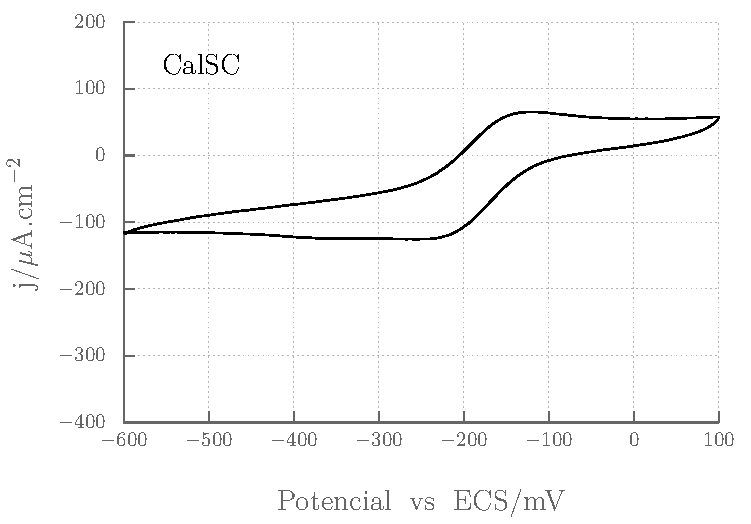
\includegraphics[width=\textwidth]{Graficos/SC-accesibilidad.pdf}
				       		\caption{Voltametría Cíclica sobre \pdmC}
				         	\end{subfigure}
				     		\caption[Accesibilidad electrodo de trabajo.]{Voltametrías Cíclicas de \aminorutenio\space \SI{1}{\milli\Molar} sobre Au recubierto con \pdm\space con una velocidad de barrido \SI{50}{\milli\volt\per\second} utilizando como referencia ESC.}
				     		\label{fig:accesibilidad}
				     		\end{figure}
	
	 \subsection{Método simplificado}

		 	De todos los tratamientos pos-depósito, se denomina método simplifcado a aquel que sigue los procedimientos establecidos en la literatura para eliminar el surfactante sin recurrir a la calcinación.\cite{Angelome2008,Calvo20210,Calvo2010,Fuertes2009} El proceso consiste en estabilizar las \pdm\space a \SI{130}{\celsius} durante \SI{1}{\hour} y luego extraer el surfactante en reflujo de 2-propanol durante \SI{15}{\minute}. 
			
			En el análisis por microscopía se aprecia que las \pdmF\space sometidas a éste tratamiento se adhieren correctamente en ambos sustratos, quedan bien estructuradas, sin grietas ni discontinuidades y se obtienen poros uniformes en tamaño y con estructuras de orden local (figura \ref{fig:Microscopia_F127_simplificado}). Las \pdmC\space sobre silicio también adhieren bien y no presentan grietas, mientras que sobre Au presentan grietas y discontinuidades en su estructura (figura \ref{fig:Microscopia_CTAB_simplificado}), lo cual se adjudica al hecho de la adsorción del bromuro sobre el Au, tema que ya fue discutido en la sección \ref{sec:adherencia}, pág. \pageref{sec:adherencia}. 
			
			La caracterización por elipsoporosimetría para las \pdmF\space resultó en una isoterma tipo IV con histéresis H5 para las \pdmC\space y tipo IV con histéresis H2 para las \pdmF\cite{Thommes2015}. Los sistemas estructurados con CTAB presentan una porosidad del 40\% aproximadamente, con una histéresis pequeña entre las ramas de adsorción y desorción de la isoterma. Esto posiblemente signifique, que no hay prácticamente diferencia entre el tamaño de poro y cuello (figuras \ref{fig:CTAB_simplificado_EPA}  y \ref{fig:CTAB_simplificado_PSD}). Este diámetro de poro pequeño se puede atribuir a que el surfactante ha sido sólo parcialmente eliminado de la estructura, estrechando el tamaño de poro hasta hacerlo prácticamente igual tamaño de los cuellos.
			En el caso de los sistemas \pdmF\space la adsorción de agua se produce en una única etapa mientras que la desorción ocurre a dos valores de presión diferentes, a P/P$_s=0,65$ y a P/P$_s=0,45$ (figura \ref{fig:F127_simplificado_EPA_2}). 

			Thielemann \cite{Thielemann2011} y Groen\cite{Groen2003} proponen que este comportamiento se produce al desorber el agua ocluida en poros, que están más o menos <<bloqueados>> por el diámetro de los cuellos, tal como se ejemplefica en la figura \ref{fig:thielemann}. Al producirse la desorción del agua a través de cuellos de distinto tamaño, la fuerza  necesaria para vencer la tensión superficial debe ser mayor, desorbiendo a menor P/P$_s$ cuanto menor sea el diámetro de los cuellos; tal como predice la ecuación de Kelvin (ver ecuación {\ref{eq:kelvin}). Esta observación se repite para varios de los tratamientos practicados e indica una población de cuellos con una doble distribución de tamaño (figura \ref{fig:F127_simplificado_PSD}). Esto sugiere dos posibilidades: 1) la existencia de dos sistemas porosos no conectados entre sí, o 2) falta de condensación en el sistema porosos con cuellos o poros medianamente ocluidos por sílice parcialmente condensada.

			%Grafico de Thielemann
			\begin{figure}[th]
		 	   	    \begin{subfigure}[t]{0.49\textwidth}
			       	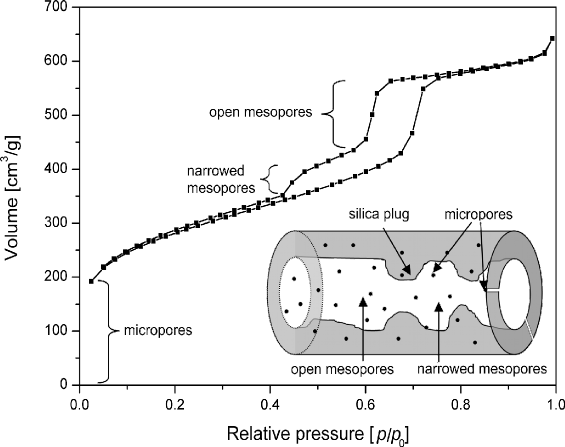
\includegraphics[width=0.90\textwidth]{Graficos/Doble-distr.png}
			       	\caption{Efecto de poros bloqueados en silice calcinada estructurada con Pluronic 123.}
			       	\label{fig:thielemann}
			   		\end{subfigure}
			   		\begin{subfigure}[t]{0.49\textwidth}
			   	    \includegraphics[width=\textwidth]{Graficos/SI_F127_simplificado_EPA.pdf}
			   	    \caption{Isoterma de adsorción/desorción de agua realizada por EPA para una \pdmF.}
			   		\end{subfigure}
					 \caption[Microscopías \pdmF\space tratamiento simplificado.]{Isotermas obtenidas para sílice mesoporosa con poros bloquedados. (a) Isoterma extradida de la publicación de Thielemann\cite{Thielemann2011} y, (b) isoterma para sistemas \pdmF\space condensadas y extraídas por el métodos simplificado.}
					 \label{fig:F127_simplificado_EPA_2}	
				     \end{figure}

			 \pagebreak En los espectros de IR, para ambos sistemas de poros (figuras \ref{fig:IR_CTAB_simplificado} y \ref{fig:IR_F127_simplificado}), se observa, entre otras, el típico acoplamiento TO$_3$-LO$_3$ que resultan en un hombro a \SI{1180}{\cm^{-1}}} indicativo de una estructura porosa\cite{Innocenzi2003}. También se ha estimado el grado de condensación en función de la relación en la intensidad de las bandas para $\nu_{\text{Si-O-Si/}}\nu_{\text{Si-OH}}$ y el porcentaje de extracción del surfactante siguiendo la intensidad de la banda para el estiramiento C-H. Como se discutirá más adelante, ésta vibración puede no sólo estar asociada al surfactante sino a la esterificación de grupos etóxidos con silanoles superficiales durante el proceso de extracción alcohólica.

			 Todos los resultados, para este y todos los tratamientos, se encuentran resumidos en la tabla \ref{tabla:resultados}.

	 \subsection{Método prolongado}

	 	 Este tratamiento se basó en prolongar el tiempo de condensación. Luego de la estabilizar las \pdm\space en cámara de humedad ($t=$\SI{1}{\hour}50 \% HR) se colocó en horno a \SI{130}{\celsius} por el término de 7 días, luego se llevó a cabo la extracción del surfactante. La elección de un período de 7 días se debe a que experimentos realizados por 1,2 y 5 días resultaban en sistemas porosos poco estables. Luego, con el propósito de estandarizar y sistematizar los experimentos y procesos de este trabajo se utilizó esté período como tiempo estándar de condensasción.

	 	 Los resultados de este proceso llevaron a depósitos homogéneas sobre silicio, sin discontinuidades ni grietas y con poros bien formados para ambos surfactantes. Cuando se utilizó Au como sustrato, sólo se obtuvieron películas de buen aspecto cuando se las estructuró con F127. Para las estructuradas con CTAB se observaron grietas y sectores enteros completamente desprendidos de los electrodos. Nuevamente, al igual que en el tratamientos anterior, este hecho sugiere que la adsorción de las micelas de CTAB al oro impiden la adhesión de las \pdmC\space a los electrodos (figuras \ref{fig:Microscopia_F127_prolongado} y \ref{fig:Microscopia_CTAB_prolongado}).

	 	 Respecto de la caracterización por EPA, para \pdmF, se observa la misma distribución de <<doble cuello>> o poros bloqueados que en el caso del tratamiento simplificado (figura \ref{fig:F127_prolongado_EPA}). En cambio, los sistemas \pdmC\space sometidos a este tratamiento muestran isotermas prácticamente idénticas al sistema calcinado, con poros de \SI{2,5}{\nm} y cuellos de \SI{1,9}{\nm} (figura \ref{fig:CTAB_prolongado_EPA}).

	 	 Los gráficos de espectroscopia IR para ambos sistemas de poros, F127 y CTAB (figuras \ref{fig:IR_F127_prolongado} y \ref{fig:IR_CTAB_prolongado}), muestran que la extracción fue exitosa. Si bien en el caso de las \pdmC\space se ve todavía una pequeña cantidad de surfactante, la cantidad relativa al no extraído es mucho menor que en el tratamiento simplificado, indicando que la extracción fue mayor. La condensación también se ha mejorado, respecto del tratamiento anterior, tal como indica el aumento relativo de la vibración correspondiente al estiramiento Si-O-Si, lo cual sugiere una maduración de la estructura porosa debido a la elongación en el tiempo de condensación. Los valores porcentuales de ambas observaciones se pueden consultar en la tabla \ref{tabla:resultados}.

	 \subsection{Método de alto vacío}\label{sec:trat-vacio}

	     Luego del éxito parcial del tratamiento prolongado, donde se obtuvieron películas homogéneas y con arreglos de poros bien formados y con estructuras comparables a la de las películas mesoporosas calcinadas\cite{Mogilnikov2002,Fuertes2008,Rothen1945}, se realizó un tratamiento similar, en cuanto a duración y temperatura (7 días a \SI{130}{\celsius}), pero colocando las muestras en alto vacío, a \SI{e-5}{\milli\bar}.

		 El motivo de llevar a cabo este tratamiento fue abastecer al sistema de calor, durante un período tiempo, para darle oportunidad de relajar y estabilizar el cristal líquido y, a la vez, aplicando vacío, desplazar el equilibrio de la reacción  \ref{eq:vacio} según el principio de Le Chatelier\cite{Atkins2006}, removiendo productos de reacción volátiles (H$_2$O y alcoholes) y así favorecer la condensación del óxido.\cite{Zhuravlev2000}

	 		\begin{equation}
				 \schemestart 
				 Si-OH + X-O-Si 
				 \arrow{->[\scriptsize{T=\SI{130}{\celsius},P=\SI{e-5}{\milli\bar}}][\scriptsize{X=H,CH$_3$CH$_2$}]}[0,2.5] 
				 Si-O-Si + X-OH $\hspace{-0.1cm}\Big\uparrow$
				 \schemestop
				 \label{eq:vacio}
				 \end{equation}
				
		 Para sistemas \pdmF, las microscopías ópticas muestran películas homogéneas, sin discontinuidades ni grietas mientras que las imgagenes de MEB revelan la presencia de nanoporos sobre ambos sustratos, silicio y oro, con poros de \SI{9}{\nm} de diámetro (ver figura \ref{fig:Microscopia_F127_vacio}). Respecto de las películas estructuradas con CTAB, presenta el mismo comportamiento que en los casos anteriores: se observa un depósito homogéneo y sin grietas cuando se depositan sobre silicio, pero se observan discontinuidades y grietas cuando se depositan sobre Au \ref{fig:Microscopia_CTAB_vacio}.

		 La isoterma de adsorción/desorción de H$_2$O muestra que desaparece la doble distribución de cuellos que se observó en los tratamientos anteriores para las películas estructuras con F127 (figuras \ref{fig:F127_vacio_EPA} y \ref{fig:F127_vacio_PSD}). El resultado es una isoterma tipo IV con histéresis H2, propia de sistemas con poros monodispersos uniformemente distribuidos, alcanzando un índice de refracción de $n=1,25$ (a P/P$_s$=0\%) y una porosidad de $38\%$, valores próximos a los de un sistema calcinado. A su vez, para \pdmC, el resultado por PEA es una isoterma que devuelve una porosidad (44 \%) y un índice de refracción ($n=1,393$) prácticamente igual al del calcinado (figura \ref{fig:CTAB_vacio_EPA}) con una distribución de tamaño de poros y cuellos (figura \ref{fig:CTAB_vacio_PSD}) comparable con la reportada por Boissiere\cite{Boissiere2005}.

		 De los espectros IR  (figuras \ref{fig:IR_F127_vacio} y \ref{fig:IR_CTAB_vacio}) se puede concluir que que la extracción del surfactante (ya sea para las películas estructuradas con F127 o estructuradas con CTAB) fue buena, pero no total, obteniendo valores de extracción por encima del 85\%. Para ambos sistemas la relación de intensidades $\nu{\text{Si-O-Si/}}\nu{\text{Si-OH}}$, así como un ángulo de contacto alto, demuestran que se trata de una estructura porosa con pared bien condensada. Los valores se encuentran en la tabla \ref{tabla:resultados}.

		 Este método fue el mas utilizado a lo largo de la tesis, debido a la reproducibilidad de los buenos resultados que se obtuvieron, tanto para la condensación como para la extracción, así como en la distribución espacial de los poros y accesibilidad al electrodo. Es por ellos que en un estadio más avanzado de la tesis se extendió su aplicación a películas de óxidos mixtos circonio/silicio utilizando tanto F127 como Brij58. Este último surfactante, como se señaló anteriormente, se utilizó en reemplazo del CTAB debido a los problemas de adherencia sobre Au de este (consultar sección \ref{sec:adherencia}). Con ambos surfactantes se lograron sintetizar películas uniformes sin grietas ni discontinuidades (figura \ref{fig:Microscopia_ZrSi_vacio}). Los voltagramas de las figura \ref{fig:accesibilidadZr} muestran los resultados de adsorber \aminorutenio\space \SI{1}{\milli\Molar} en sistemas mixtos \pdmZ\space y \pdmZB\space utilizando F127 y Brij58 como molde para los poros, donde se demuestra la accesibilidad y el poder de adsorción de ambos sistemas con distinto tamaño de poro.

		 	\begin{figure}[th]
		       \begin{subfigure}[t]{0.495\textwidth}
		       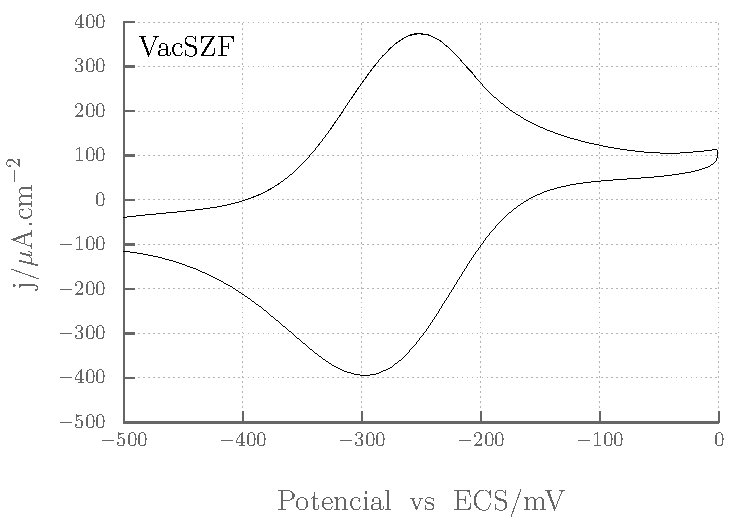
\includegraphics[width=\textwidth]{Graficos/SZF-accesibilidad.pdf}
		       \caption{Voltametría Cíclica sobre \pdmZ\space correspondiente al ciclo número 95.}
		       	\end{subfigure}
		       	\begin{subfigure}[t]{0.495\textwidth}
		       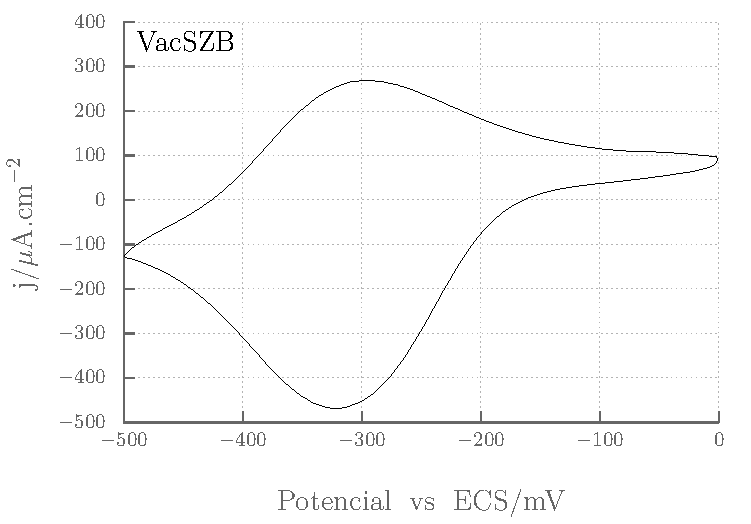
\includegraphics[width=\textwidth]{Graficos/SZB-accesibilidad.pdf}
		       \caption{Voltametría Cíclica sobre \pdmZB\space correspondiente al ciclo número 105.}
		   	\end{subfigure}
	     	\caption[Accesibilidad electrodo de trabajo sistemas mixtos Zr/Si.]{Voltametrías Cíclicas de \aminorutenio\space \SI{1}{\milli\Molar} a una velocidad de barrido \SI{50}{\milli\volt\per\second} sobre electrodos de Au recubierto con \pdm\space por el método de alto vacío. a) \pdm\space mixtas Zr/Si estructuras con F127 y, b)  mixtas Zr/Si estructuras con Brij58.}
			\label{fig:accesibilidadZr}
		     \end{figure}


		 %muestra que las pdm basadas en circonico/Silice sintetizadas opir este método tienen buena accesibilidad y su capacidad de adosrocion es similar. Estos temas son materia del capitulo siguiente y se discuten allí en profundidad.

	 \subsection{Método ácido}

	 	 Algunos autores proponen que un medio fuertemente ácido (pH$<1$) favorece la hidrólisis del alcóxido y la condensación de los grupo siloxano \cite{Soler-Illia2011,Doshi2000a,Huo1996,Boissiere2000,Beck1992}. Las películas depositadas, estabilizadas en cámara de humedad y  parcialmente condensadas a \SI{130}{\celsius}, tal como se explica en la sección \ref{sec:cond_y_extr}, pág. \pageref{sec:cond_y_extr}, fueron expuestas a una atmósfera de HCl durante \SI{15}{\minute}. 

		 En las microscopias para las \pdm\space sometidas a este método (ya sean estructuradas con F127 como con CTAB) se observan grietas y discontinuidades cuando se depositaron sobre electrodos de Au (figuras \ref{fig:Microscopia_F127_acido} y \ref{fig:Microscopia_CTAB_acido}). Este hecho se ha atribuido a una condensación rápida, catalizada por el medio extremadamente ácido. Al no presentar buena adherencia sobre el sustrato, las películas de sílice se contraen en todas las direcciones, y no solo en la dirección normal a la superficie, como ocurre en las \pdm\space depositadas sobre silicio, donde las fuerzas de adherencia al sustrato priman por sobre las fuerzas contracción en el plano\cite{Sakatani2006,Boissiere2005,Guillemin2010}. En ese caso las películas quedan bien formadas y homogéneas en toda el área de la muestra para ambos surfactantes. Se ha observado por microscopía electrónica que para los sistemas \pdmF\space (\ref{fig:Microscopia_F127_acido}) los  poros están casi unidos formando una especie de poro elongado, propio de una estructura \textit{p6mm}\cite{GonzalezSolveyra2017}. 
	
		 Esta morfología superficial de poros elongados se corroboró por PEA (figura \ref{fig:F127_acido_EPA}). Allí se observa, en la isoterma de adsorción/desorción de agua, una doble distribución de cuellos donde predominan cuellos de diámetro grandes, casi del mismo tamaño que los poros, coincidiendo con la observación por microscopía electrónica.
		 Como se puede apreciar en la tabla \ref{tabla:resultados}, las dimensiones de los poros, medidos por por ambas técnicas, dan valores diferentes. Esta discrepancia posiblemente se deba a que la medición por PEA no resulte del todo apropiada para este tipo de estructuras de poros elongados, no esféricos, suposición necesaria para el calculo de las dimensiones de los poros. En cambio, mediante MEB se puede extrapolar la curvatura para simular una esfera y medir los poros, obteniéndose valores de diámetro similares a los de las \pdmF sintetizadas por otros métodos.

		 La isoterma de adsorción/desorción de agua para \pdmC\space muestra que se trata de sistemas con una porosidad del 38\% y un índice de refracción $n=1.23$, al igual que en el caso del F127 apenas superior que en el caso de lo sistemas calcinados.
		
		 En lo referente a la etapa de extracción, se observa por espectroscopia IR, que fue efectiva para ambos sistemas de poros, alcanzando un alto porcentaje de extracción, $91,5$\% para CTAB y $85,7$\% para F127 (figuras \ref{fig:IR_CTAB_acido} y \ref{fig:IR_F127_acido}).  	
				
	 \subsection{Método alcalino}

	 	 El último de los tratamientos experimentados en pos de conseguir depositar y condensar peliculas mesoporosa de óxido de silicio a bajas temperatura fue el tratamiento en medio básico. Análogamente al realizado en medio ácido, se basa en someter a las películas a un medio de pH extremo (pH$>12$), el cual, según algunos autores \cite{Soler-Illia2011,Huo1996,Ichinose2002,GonzalezSolveyra2017}, cataliza los procesos de hidrólisis del TEOS. En este caso las películas, luego de la estabilización en humedad, fueron colocadas en una atmósfera de NH$_3$ durante \SI{15}{\minute}. 

		 Los depósitos obtenidos sobre Au presentan grandes grietas y zonas muy fraccionadas para ambos sistemas porosos, \pdmF\space y \pdmC. Esta observación se atribuye nuevamente a la violenta condensación catalizada por el medio, en este caso fuertemente alcalino. Sobre silicio las \pdm\space resultaron en depósitos homogéneos y de buen aspecto tanto por microscopia óptica como electrónica (figuras \ref{fig:Microscopia_F127_basico} y \ref{fig:Microscopia_CTAB_basico}).

		 En las elipsoporosimetría realizadas, se observa para el sistema \pdmF\space una doble distribución de cuellos muy similar a la obtenida por el tratamientos en medio ácido, pero en este caso el índice de refracción fue de $n=1.22$ (a P/P$_s$ = 0) el cual es prácticamente idéntico al que presentan los sistema calcinado (ver figura \ref{fig:F127_basico_EPA} y tabla \ref{tabla:resultados}). Para poros estructurados con CTAB las mediciones por PEA muestran una isoterma tipo IV, con histérisis H1, resultando en un sistema muy poroso ($40\%$) y un índice de refracción $n=1,22$.
	
		 Los espectros IR para ambos surfactantes (figura \ref{fig:IR_CTAB_basico} para CTAB y \ref{fig:IR_F127_basico} para F127) muestran una ruptura en el aspecto del típico hombro (acoplamiento LO$_3$-TO$_3$, en \SI{1180}{\per\cm}) para estructuras de sílice mesoporosas \cite{Olsen1989,Innocenzi2003,Angelome2008}. Esto sugiere un colapso de la organización de poros en la nanoescala, debido a la disolución parcial de la sílice, catalizada por el medio básico. Si bien el medio básico acelera la hidrólisis del TEOS, también aumenta la tasa de disolución del SiO$_2$.\cite{Mazer1994,Niibori2000,Gorrepati2010}

	 \subsection{Comparación de resultados de los tratamientos pos-síntesis}
	 		
	 		En la tabla \ref{tabla:resultados} se comparan los resultados de las caracterización de las \pdm\space obtenidas por cada uno de los tratamientos pos-depósito. La información organizada en forma concisa y sistemática resume los resultados de microscopia (óptica, MEB y FIB), elipsoporosimetría, angulo de contacto, FTIR, electroquímica para cada sistema en particular. Respecto de los resultados por microscopia se destaca que el visto bueno es para aquellas películas homogéneas en superficies extensas, sin grietas ni discontinuidades tanto a escala macro como microscópica. La señal EQ positiva se refiere a pruebas de \pdm\space homogéneas sobre electrodos de Au, en las cuales la sonda puede difundir a través de la película hasta alcanzar la superficie del electrodo.

	 		%Se presentan en la tabla \ref{tabla:resultados} todos los resultados, obtenidos para cada sistema de poros, \pdmF\space y \pdmC, por cada una de las técnicas de caracterización empleadas. 

	 		%La tabla se compone de varias columna; una para microscopía donde se coloca el aspecto que presentan las diferentes \pdm\space tanto sobre oro como sobre silicio; otra con resultados de poroelipsometría ambiental y los valores que extraídos de las isotermas: diámetro de poro ($\varnothing_p$), de cuello($\varnothing_c$), porosidad (\%P), espesor ($e$) e índice de refracción de la pared ($n$); otra para los resultados de FTIR donde se ha volcado el porcentaje de extracción del surfactante y la relación de intensidad picos $\nu_{\text{Si-O-Si/}}\nu_{\text{Si-OH}}$; una más para la accesibilidad al electrodo de sondas EQ; otra para el ángulo de contacto ($\theta$) y una última reservada para observaciones generales.  
	 
	 		 \begin{table}[p]
			 \caption[Comparación de resultados \pdm]{Resumen de resultados obtenidos por cada una de las técnicas de caracterización, para cada uno de los métodos pos-depósito aplicados a \pdm. Tanto los diámetros ($\varnothing$) como los espesores ($e$) están expresando en nm.}
			 \label{tabla:resultados}
		 	 \begingroup
		 	 \subcaption{Parte A: Microscopía, elipsoporosimetría y ángulo de contacto.}
			 \endgroup
			 \addtolength{\tabcolsep}{-2.7pt} 
			 \begin{tabular}{l c@{\hspace{5.9mm}} c c c@{\hspace{4.3mm}} c c c c@{\hspace{6.6mm}} c c@{\hspace{2pt}} c c c c@{\hspace{6.25mm}} c}
			 \toprule
			 Técnica & &\multicolumn{6}{c}{Microscopia}& &\multicolumn{5}{c}{Elipsoporosimetría} &  & AC \\
   			 Sustrato& &\multicolumn{2}{c}{Si}& &\multicolumn{3}{c}{Au}& &\multicolumn{5}{c}{Si}&  & Si \\ 
    			 	 & &\faEye&$\varnothing_p$& &\faEye&$\varnothing_p$&$e$& &$\varnothing_p$&$\varnothing_c$&\%P&$e$&$n(\lambda)^\mathsection$& &$\theta^\circ$\\ \midrule 

    		 CalSC & &\checkmark&-   & &\xmark    &-  &258& &2,5 & 2,0 & 42 & 265 & 1,384 & & 33,2 \\ 
  	 	     CalSF & &\checkmark&9,0 & &\checkmark&9,1&215& &8,2& 4,4 & 38 & 207 & 1,391 & & 20,0 \\ \midrule
  	 	     SimSC & &\checkmark&-   & &\xmark    &-  &-& & 2,2& 2,0 & 30 & 308 & 1,389 & & 41,2 \\ 
			 SimSF & &\checkmark&7,8 & &\checkmark&7,0&-& &7,5 & \hspace{1.5mm}3,9$^\dagger$& 30 & 211 & 1,390 & & 36,4 \\ \midrule
			 ProSC & &\checkmark&-   & &\xmark    &-  &-& & 2,5& 2,0 & 41 & 338 & 1,375 & & 44,5 \\ 
			 ProSF & &\checkmark&8,1 & &\checkmark&8,5&-& &8,0 & \hspace{1.5mm}4,0$^\dagger$  & 39 & 212 & 1,381 & & 22,7 \\ \midrule
			 VacSC & &\checkmark&-   & &\xmark    &-  &-& &2,2 & 1,7  & 44 & 381 & 1,393 &&  65,5 \\ 
			 VacSF & &\checkmark&8,2 & &\checkmark&8,2&201& &9,0 & 4,0  & 38 & 223 & 1,383 & & 42,5 \\
			 VacZSF& &\checkmark&8,5 & &\checkmark&-  &-& & -  &  -	 & -  &  -  &    -  &  &  -  \\ 
			 VacZSB& &\checkmark&-   & &\checkmark&-  &-& & -  &  -	 & -  &  -  &    -  &  &  -  \\ \midrule
			 ÁciSC & &\checkmark&-   & &\xmark    &-  &-& &2,0 & 1,6  & 37 & 340 & 1,386 & &46,0 \\ 
			 ÁciSF & &\checkmark&8,2 & &\xmark    &-  &-& &5,7 & \hspace{1.5mm}2,1$^\dagger$  & 31 & 191 & 1,399 & & 28,2 \\ \midrule
			 AlcSC & &\checkmark&-   & &\xmark    &-  &-& &2,3 & 1,6  & 46 & 383 & 1,396 & & 47,6 \\ 
			 AlcSF & &\checkmark&8,3 & &\xmark    &-  &-& &8,0 & \hspace{1.5mm}2,1$^\dagger$ & 32 & 225 & 1,374 &  & 24,5 \\
			\bottomrule
			\end{tabular}
		    \begingroup
		    \subcaption{Parte B: Espectroscopía IR, accesibilidad de sondas EQ y observaciones.}
			\endgroup
			\begin{tabular}{l@{\hspace{8.2mm}} c c@{\hspace{6.25mm}} c@{\hspace{6.25mm}} l@{\hspace{3.7mm}}} 
			\toprule
				 \multirow{2}{*}{Método}& \multicolumn{2}{c}{FTIR} & Señal EQ & Observaciones generales\\
    			   		 & $\frac{\nu{\text{Si-O-Si}}}{\nu{\text{Si-OH}}}$ & \%$_{\text{ext}}$  \\ \midrule

    			 CalSC   & 1,08  & 100  & \checkmark & falta de adherencia en Au  \\ 
  	 	         CalSF   & 0,77  & 100  & \checkmark &   \\ \midrule
  	 	         SimSC   & 0,67  & 72,7 & \xmark & falta de adherencia en Au  \\ 
			     SimSF   & 0,53  & 70,4 & \xmark & doble cuello \\ \midrule
				 ProSC   & 0,80  & 87,7 & \xmark & falta de adherencia en Au  \\ 
				 ProSF   & 0,78  & 97,0 & \xmark & doble cuello \\ \midrule
				 VacSC   & 0,88  & 87,5 & \checkmark & falta de adherencia en Au  \\ 
				 VacSF   & 0,78  & 88,0 & \checkmark &   \\ 
				 VacZSF  &   -   &   -  & \checkmark &   \\ 
				 VacZSB  &   -   &   -  & \checkmark &   \\ \midrule
				 ÁciSC   & 0,80  & 91,5 & \xmark & falta de adherencia en Au  \\ 
				 ÁciSF   & 0,81  & 85,7 & \xmark & doble cuello, poros <<elongados>>  \\ \midrule
				 AlcSC   & 0,99  & 94,4 & \xmark & \multirow{2}{*}{pérdida de la estructura porosa} \\ 
				 AlcSF   & 0,98  & 91,2 & \xmark &   \\
			\bottomrule
			\end{tabular}\vspace*{2pt}
			\footnotesize{$^\mathsection$ Valores de $n$ calculados para las paredes de los sistemas mesoporosos a $\lambda=$\SI{600}{\nm}; índice de refracción de SiO$_2$ por sol-gel, $n=1,45$.} \\
			\footnotesize{$^\dagger$ Sistemas con doble distribución de cuellos, se reporta la población más abundante.}\\
			\end{table}					 	  

			
\section{Discusión sobre los métodos}
		
			Luego de depositar, sintetizar, llevar a cabo los tratamientos y caracterizar las distintas películas, en esta sección se presenta una discusión general sobre los resultados obtenidos para cada uno de los métodos. El resultado de la discusión y el análisis exhaustivo de los datos para cada tratamiento libre de calcinación, tendrá como objetivo final escoger uno o más métodos adecuados para la fabricación de sensores basados en películas mesoporosas de sílice.

	\subsection{Sobre los sustratos}

			Para utilizar las \pdm\space como sensores EQ, se deben depositar sobre un sustrato apto para reacciones electroquímicas. Podemos contar dentro de este grupo: carbono vítreo, ITO, FTO, grafito, Au y Pt entre otros. Se decidió utilizar Au, depositado por pulverización catódica sobre obleas de silicio para obtener electrodos de baja rugosidad. Este tipo de sustrato permite obtener señales EQ repetibles, sin interferencias ni distorsiones y comparables con aquellas en literatura.\cite{Wi2000,Bockris1974} De esta forma se pudo focalizar la atención en los fenómenos de transporte a lo largo de las membranas mesoporosa y no en las distorsiones de la señal que podría causar otro tipo de electrodo, debida a efectos de alta rugosidad o de una cinética de electrodo lenta.
		
		    En los electrodos con un diseño transferido se utiliza una capa dieléctrica de SiO$_2$, por lo que fue necesario realizar depósitos sobre silicio para determinar la compatibilidad con estos sustrato. Además estos depósitos fueron de suma importancia llevar cabo numerosas caracterizaciones (que sobre Au no eran posibles), entender las bases de algunos comportamientos y comparar con la literatura.\cite{Innocenzi2013}

			Hubo dos métodos en particular, el tratamiento en medio ácido y el tratamiento en medio básico, que mostraron el mismo comportamiento independientemente del surfactante utilizado. Ambos resultaron en la aparición de grietas a lo largo de toda la película sobre sustrato de Au. Esto es resultado de dos factores combinados; la baja adherencia sobre sustrato de Au (a los sistemas con CTAB se le suma la adsorción del surfactante al sustrato) y la rápida condensación catalizada por el medio, ya se sea ácido o básico. Esto lleva a una contracción en todas direcciones ya que la fuerza de adherencia al Au es menor que la fuerza de contracción en el plano de la película, lo cual genera las discontinuidades y grietas en las \pdm. No ocurre lo mismo cuando el sustrato es silicio, donde la adherencia entre la película y el sustrato es fuerte. En este caso la contracción es uniaxial (como es lo habitual para sistemas calcinados) y sólo ocurre en el eje normal a la superficie, resultando en depósitos continuos y homogéneos para cada uno de los métodos practicados.

			Los sistemas que usaron CTAB y fueron depositados sobre Au presentaron grietas, fracturas y discontinuidades en todos los casos como ya fue mencionando. Esto es consecuencia de la adsorción superficial del Br sobre el Au que disminuye la adherencia de las \pdm\space sobre los electrodos. 

			Tanto los sistemas puros \pdmF, como los mixtos Zr/Si, \pdmZ\space y \pdmZB, depositados por el método de alto vacío resultaron en películas homogéneas tanto en espesor como en superficie y con buena accesibilidad al electrodo.

	\subsection{Sobre la condensación}

		Una de las dos técnicas utilizadas para evaluar la condensación de las \pdm\space fue elipsoporosimetria ambiental (PEA), mediante la cual construye una isoterma donde se gráfica índice de refracción en función de la presión parcial de H$_2$O. De dicha técnica se puede extraer el índice de refracción del SiO$_2$ de las \pdm, ponderando su porosidad, según la aproximación de Bruggeman, la cuál debe satisfacer la ecuación \ref{eq:bruggeman} \cite{Bruggeman1935} (los detalles se puede consulta en la sec. \ref{sec:elipso}, pág. \pageref{sec:elipso}) Este valor, comparado con el sistema calcinado, nos da una idea de cuán condensada está la película. También se obtienen información cuantitativa sobre el volumen poroso de las películas, información estadística sobre el diámetro de los poros y cuellos. En las figuras \ref{fig:todos_EPA_F127} y \ref{fig:todos_EPA_CTAB} se comparan las isotermas obtenidas para cada uno de los sistemas, estructurado con CTAB y con F127. Y en la figura \ref{fig:histogramas} se presentan histogramas comparativos relativos a las magnitudes mas relevantes para llegar a conclusiones sobre los métodos experimentados.

		Todos los métodos ensayados para sistemas \pdmF\space y \pdmC resultaron en películas porosas. Sin embargo en algunos en los que se empleó F127 como surfactante (simplificado, ácido y básico) presentaron doble distribución de cuellos, sugiriendo sistemas con doble tamaños de cuellos o sistemas condensados parcialmente por sectores no conectados entre sí, con su propia y característica distribución de poros y cuellos. Para todos los tratamientos, los índices de refracción dan valores similares con óxidos mesoporosos calcinados, indicando una condensación similar a éstos. 


			\begin{figure}[bh!]
		 	   	   \begin{center}
		 	   	   \includegraphics[width=\textwidth]{Graficos/SI_CTAB_todos_EPA.pdf}
			   	   \caption[Comparación PEA tratamientos alternativos (CTAB)]{Comparación de las isotermas para todos los tratamientos pos-depósito para \pdmC\space. Destacan los altos índices de refracción para los tratamientos simplificado y en medio ácido.}
				   \label{fig:todos_EPA_CTAB}	
				   \end{center}
				   \end{figure}
			
			\begin{figure}[th!]
		 	   	   \begin{center}
		 	   	   \includegraphics[width=\textwidth]{Graficos/SI_F127_todos_EPA.pdf}
			   	   \caption[Comparación PEA tratamientos alternativos (F127)]{Comparación de las isotermas para todos los tratamientos pos-depósito para \pdmF\space. Se destacan la doble distribuciones de cuellos para algunos de ellos.}
				   \label{fig:todos_EPA_F127}	
				   \end{center}
				   \end{figure}	

				   \begin{figure}[ht!]
				 	   	    
				 	   	    \begin{subfigure}[t]{0.5\textwidth}
				        	\includegraphics[width=\textwidth]{Graficos/histogramas-poros.pdf}
				       		\end{subfigure}
				         	\begin{subfigure}[t]{0.5\textwidth}
				        	\includegraphics[width=\textwidth]{Graficos/histogramas-cuellos.pdf}
				       		\end{subfigure}
				         	 \begin{subfigure}[t]{0.5\textwidth}
				        	\includegraphics[width=\textwidth]{Graficos/histogramas-volumen.pdf}
				       		\end{subfigure}
				         	\begin{subfigure}[t]{0.5\textwidth}
				        	\includegraphics[width=\textwidth]{Graficos/histogramas-indice.pdf}
				       		\end{subfigure}
				     		\caption[a]{Comparación de las magnitudes, extraídas del análisis por EPA, mas relevante para comparar el grado de condensación de las películas delgadas mesoporosas en base sílice, estructuradas con F127 (SF) y CTAB (SC).}
				     		\label{fig:histogramas}
				     		\end{figure}
		
		La otra técnica utilizada para evaluar la condensación fue espectroscopia IR. Para ello se calculó la relación existente entre la intensidad de picos correspondiente a las vibraciones $\nu{\text{Si-O-Si}}$ y $\nu{\text{Si-OH}}$ \cite{Pai1986,Innocenzi2003}. Un número mayor indica mayor cantidad de enlaces Si-O-Si, por lo tanto mayor grado de condensación. Se observa en la tabla \ref{tabla:resultados} que los mayores valores corresponden a los sistemas calcinados y los menores a los sistemas en lo que solo se estabilizó a \SI{130}{\celsius} (método simplificado). Los valores obtenidos para el resto de los tratamientos se encuentran próximos a los valores correspondientes a sistemas calcinados, lo cual sugiere un buen grado de condensación.  Otra banda importante es el hombro de LO$_3$ (\SI{1180}{\per\cm}) formado a mayores frecuencias de TO$_3$, característico de estructuras porosas de SiO$_2$. Esta señal se debe al acoplamiento longitudinal/transversal de los modos TO$_3$ y LO$_3$ ocasionada por la dispersión de la luz en la red porosa, que estimula el modo longitudinal el cual habitualmente no se excita cuando se mide en modo trasmisión\cite{Innocenzi2003,Lange1990,Lange1989}. La ausencia de este acoplamiento sugiere un sistema poco poroso o más denso. Esto sugiere, junto a otros indicios, al colapso parcial de la estructura porosa. En la tabla \ref{tabla:resultados} se muestran los valores cuantitativos respecto de estas bandas.	
			

	\subsection{Sobre la extracción}

		Al utilizar métodos alternativos a la calcinación se requirió una etapa de extracción para eliminar el surfactante. En todos los caso se llevó a cabo en 2-propanol a reflujo. Si bien fue exitosa en la mayoría de los casos, con valores de extracción por encima del 85\%, siempre se observa una pequeña banda correspondiente a la vibración C-H en el IR. Dicha banda puede provenir tanto del surfactante como de intercambiar el hidroxilo por propanol según:
			\begin{equation}
				 \schemestart 
				 Si-OH + OH-CH$_2$CH$_3$ 
				 \arrow{<=>}[0,1.5] 
				 Si-O-CH$_2$CH$_3$ + H$_2$O
				 \schemestop
				 \label{eq:prolilo}
				 \end{equation}
				 \begin{figure}[ht!]
			\begin{center}
			\includegraphics[width=0.85\textwidth]{Graficos/IR_F127_vacio_AGUA.pdf}
			\caption[FTIR extracción agua ácida.]{IR para cada etapa de eliminación del surfactante correspondiente a una \pdmF\space sintetizada por el método de alto vacío.}
			\label{fig:IR_agua}
			\end{center}
			\end{figure}

			
		Por este motivo, luego de la extracción con 2-propanol, se realizó un enjuague de las muestras con H$_2$O acidificada con HCl (pH$\approx 2$) para poder completar la extracción, ya sean residuos de surfactante o propanol ligado.
				
		En la figura \ref{fig:IR_agua} se muestra una película delgada de sílice, estructurada con F127, y preparado por el método de alto vacío. Allí donde se comparan tres espectros IR para cada etapa; la película antes de extraer el surfactante, luego de extraerlo con 2-propanol y, luego de extraerlo con el alcohol y seguido de un enjuague en agua acidificada. Se ve como con el enjuague en agua ácida disminuye la señal correspondiente a la vibración C-H, que aparece ya sea por restos de surfactante y/o de la esterificación del 2-propanol.

	\subsection{Sobre la respuesta electroquímica}\label{sec:acc_eq}

	  Una parte fundamental en la fabricación de las \pdm\space y su potencial uso para sensores electroquímicos es la accesibilidad de moléculas dentro de la red porosa. Ya se demostró, en la sección \ref{sec:acc}, pág. \pageref{sec:acc} que el \aminorutenio\space es capaz de difundir en sistemas calcinados a través de los poros hasta la superficie del electrodo, donde tiene lugar la reacción electroquímica. Se debe evaluar, entonces,  la accesibilidad en sistemas de poros no calcinados. Parra ello se realizaron sendas mediciones electroquímicas sobre películas depositadas, condensadas y extraídas con el tratamiento de alto vacío, ya que es el que mostró las mejores condiciones de adherencia al Au, condensación y distribución de poros para usar en sensores EQ. 

	  		\begin{figure}[bt!]
		 	
		 	\begin{subfigure}[t]{0.5\textwidth}
		          	\includegraphics[width=\textwidth]{Graficos/Ru-F127-CNEA-Calcinado-0-1.pdf}
		          	\vspace*{-6mm}
		         	\caption{Ciclos de VC para \ru\space \SI{0.1}{\milli\Molar} sobre \pdmF\space calcinadas.}
		          	\vspace*{3mm}
		          	\label{fig:cal_01mM}
		          	\end{subfigure}
		    \begin{subfigure}[t]{0.5\textwidth}
		          	\includegraphics[width=\textwidth]{Graficos/Ru-F127-INTI-BajaT-0-1.pdf}
		         	\vspace*{-6mm}
		         	\caption{Ciclos de VC para \ru\space \SI{0.1}{\milli\Molar} sobre \pdmF\space sin calcinar.}
		      		\vspace*{3mm}
		      		\label{fig:vac_01mM}
		      		\end{subfigure}
		    \begin{subfigure}[t]{0.5\textwidth}
		          	\includegraphics[width=\textwidth]{Graficos/Ru-F127-CNEA-Calcinado-1.pdf}
		         	\vspace*{-6mm}
		         	\caption{Ciclos de VC para \ru\space \SI{1}{\milli\Molar} sobre \pdmF\space calcinadas.}
		            \vspace*{3mm}
		            \label{fig:cal_1mM}
		            \end{subfigure}
		    \begin{subfigure}[t]{0.5\textwidth}
		          	\includegraphics[width=\textwidth]{Graficos/Ru-F127-INTI-BajaT-1.pdf}
		         	\vspace*{-6mm}
		         	\caption{Ciclos de VC para \ru\space \SI{1}{\milli\Molar} sobre \pdmF\space sin calcinar.}
		    		\vspace*{3mm}
		    		\label{fig:vac_1mM}
		    		\end{subfigure}
		      	 	\caption[Voltagrama comparativo SF calcinados/alto vacío I]{Voltametrías cíclicas donde se compara la accesibilidad de una sonda electroquímica sobre \pdmF\space con dos tratamientos pos-depósito diferentes; (a) y (c) por calcinación a (\SI{350}{\celsius}) y, (b) y (d) por el método de alto vacío (\SI{130}{\celsius}, 7 días, P=\SI{e-5}{\milli\bar}). Todas las VC fueron realizadas en una solución \SI{0.1}{\Molar} de KCl a \SI{50}{\milli\volt\per\second}.}
		      		\label{fig:comp-calc-vacio}
	      \end{figure}

	  En la figura \ref{fig:comp-calc-vacio} se exponen las voltametrías cíclicas comparando \pdmF\space condensadas por calcinación y por el método de alto vacío, a dos concentraciones de sonda diferentes. Los voltagramas están compuestos por ciclos consecutivos de voltametrías cíclicas hasta llegar a un máximo donde ya no varía la respuesta. Este respuesta corresponde al ingreso y adsorción de la sonda en las \pdm, hasta llegar a la saturación. Este comportamiento es materia central del capitulo siguiente donde se lleva a cabo una profunda discusión sobre los fenómenos de transporte dentro de los poros.

      Si bien la capacidad de adsorción es prácticamente igual (la concentración dentro de los poros, determinada por el área de la curva azul de los voltagramas), ya sea que se trate del sistema calcinado o del sistema de alto vacío, el mecanismo de adsorción, hasta llegar a saturación, parece ser diferente. 

      En los sistemas calcinados la respuesta del primer ciclo (representado por la curva roja en la figura \ref{fig:comp-calc-vacio}) es comparable con la respuesta esperada en un electrodo de Au desnudo, sin recubrir. A medida que se realizan ciclos consecutivos de VC, el sistemas evoluciona en la respuesta típica de un adsorbido. Esta tendencia seta marcada con una flecha en los voltagramas de la la figuras \ref{fig:cal_1mM} y \ref{fig:cal_01mM}. En cambio, en los sistemas de alto vacío, los primeros ciclos no dan respuesta EQ, mostrando una señal chata (curva roja) , y, conforme la sonda ingresa en los poros, la respuesta aumenta y hasta ser prácticamente igual a la del sistema calcinado (marcado por la flechas en las figuras \ref{fig:vac_1mM} y \ref{fig:vac_01mM}. 

      Este comportamiento sugiere que la accesibilidad no es la misma para estos sistemas, con marcadas diferencias en la cinética de adsorción. Los calcinados son sistemas más abiertos o más comunicados, en los cuales la sonda difunde rápidamente a través de canales hasta llegar al electrodo y reaccionar desde el primer ciclo. En los sistemas condensados a bajas temperaturas la difusión de la sonda al electrodo parece esta impedida, y la respuesta aumenta conforme aumenta la concentración de sonda dentro de los poros. En resumen, en los sistemas calcinados la difusión es más rápida que la adsorción y en los de alto vacío la difusión esta impedida y solo se manifiesta señal EQ luego de varios ciclos voltamperometricos, a medida que se adsorbe, a pesar de que la capacidad final de adsorción es igual para ambos métodos.

      Esta observación ya fue observada en la tesis de Calvo\cite{Calvo20210}, donde utiliza \pdmF\space funcionalizadas con grupos aminos, no calcinados y condensados a \SI{200}{\celsius}. En dicho trabajo no se observa señal EQ para estos sistemas mientras que en sus homólogos calcinados si. Este hecho se lo atribuye a que los poros necesitan ser <<activados>> debida a una baja condensación. Aquí queda demostrado que que que en realidad se trata de una impedimento cinético debido a la condensación realizadas a T$<$\SI{350}{\celsius}.

      Esta diferencia de accesibilidad de los sistemas calcinados respectos de los sistemas de alto vacío también se hizo evidente cuando se utilizó ferroceno metanol como sonda. Esta sonda es neutra, por lo tanto no debería verse influenciada por la carga dentro de las películas. En la figura \ref{fig:fcOH_accesibilidad} se compara la respuesta de un \pdmF\space condensado y extraído por el método de alto vacío y un sistema \pdmF\space calcinado. Si bien ambos sistemas demostraron ser accesibles, los sistemas condensados a bajas temperaturas da un respuesta propia de un sistema limitado por difusión. En el capítulo \ref{chap:Electroquimica} se discute y analiza en profundidad  los resultados de transporte del ferroceno metanol en sistemas \pdmF, así como cálculos de constantes de difusión.

      		\begin{figure}[ht!]
		 	\begin{subfigure}[t]{0.5\textwidth}
		          	\includegraphics[width=\textwidth]{Graficos/Acc-FcOH-Calcinado.pdf}
		          	\end{subfigure}
		    \begin{subfigure}[t]{0.5\textwidth}
		          	\includegraphics[width=\textwidth]{Graficos/Acc-FcOH-BajaT.pdf}
		         	\end{subfigure}
		         	\caption[Voltagrama comparativo SF calcinados/alto vacío II]{Voltametrías para \fc\space \SI{1}{\milli\Molar} en \SI{100}{\milli\Molar} de KCl realizada a \SI{50}{\volt\per\second} contra ESC. Izquierda: sobre sistemas \pdmF\space calcinados. Derecha: sobre sistemas \pdmF\space condensados por el método de alto vacío y extraído con 2-propanol y agua.}
		         	\label{fig:fcOH_accesibilidad}
		    \end{figure}     	

\section{Conclusiones parciales}
	
	En este capítulo se presentaron los resultados obtenidos durante el proceso de fabricación, desarrollo y caracterización de películas delgadas mesoporosas de óxido de silicio con potencial uso en sensores electroquímicos.
	
	Los soles, precursores de las \pdm, se depositaron exclusivamente por \textit{spin-coating}, previendo la futura integración a los procesos propios de la industria electrónica. La organización espacial de los poros se llevó a cabo con tres agentes moldeantes, CTAB, Brij58 y F127, sobre diferentes sustratos: silicio, vidrio y oro. Se ajustó el espesor entre 200 y \SI{250}{\nm}, el cuál se consideró óptimo para obtener \pdm\space sin fracturas ni discontinuidades; y frente a los problemas de adherencia a los electrodos se utilizaron dos estrategias: modificación química y optimización del diseño de los electrodos. 

	Una vez adquirida la experiencia para depositar y condensar por calcinación \pdm\space sobre electrodos, con poros accesibles, sin discontinuidades y con buena adherencia, se propusieron distintos métodos pos-depósito para obtener \pdm\space a temperaturas menores a \SI{130}{\celsius}. Para ello se realizó un trabajo sistemático y metódico sobre el estudio y desarrollo de procesos pos-depósito. En total fueron cinco los procesos desarrollados: simplificado, prolongado, alto vacío, ácido y alcalino.

	Los resultados muestran que cualquiera de los métodos es plausible de ser usado para obtener \pdm, con poros accesibles, y porosidades entre 30\% y 45\%. Sin embargo, este trabajo tiene por objetivo utilizar estas películas como elemento activo permeoselectivo incorporado en sensores. Para ello no basta solo con obtener películas mesoporosas sobre silicio o vidrio (sistemas más clásicos), sino que hay que depositarlas y condensarlas sobre electrodos que permitan una detección electroquímica confiable, como Au o Pt. También es preciso mantener, durante todo el proceso de síntesis, la temperatura por debajo de los \SI{150}{\celsius} para evitar procesos difusivos, como discutiremos en el capítulo \ref{chap:Microfabricacion}.

	Las películas estructuradas con F127 mostraron dificultades a la hora de obtener distribuciones homogéneas de poro y cuello para los tratamientos simplificado, prolongado, ácido y básico. Sin embargo con tiempos de estabilización prologados y en alto vacío resultaron homogéneas en todo sentido, tanto en el depósito en sí, como en un distribución estrecha de poros y cuellos. Este hecho sugiere que el tiempo de estabilización prolongado sumado al alto vacío (que favorece la reacción de condensación) ayudan a controlar la condensación y la organización espacial de los poros, obteniendo sistemas de un buen grado de condensación con poros y cuellos uniformemente distribuidos.

	No fue posible obtener depósitos continuos sobre Au en películas estructuras con CTAB. Esto se debe a las limitaciones de adherencia sobre Au, sumado a la adsorción del surfactante catiónico sobre la superficie del mismo. A pesar de ello, los métodos desarrollados sobre silicio demostraron ser parcialmente exitosos en todos los casos. En reemplazo de CTAB y en base a la experiencia adquirida durante el desarrollo de los métodos de baja temperatura, se incorporó Brij58 en soles mixtos Zr/Si para obtener nanoporos del orden de los \SI{5}{\nm} empleando el método de alto vacío. El resultado fueron películas accesibles, homogéneamente distribuidas y de gran estabilidad frente a la disolución por el agregado de circonio. 

	De los cinco métodos desarrollados, sólo el de alto vacío resulto ser apto para utilizar indistintamente CTAB, F127 o Brij58. Este resultado resulta interesante en sí, ya que, si bien las películas con CTAB sobre Au no adhieren, es importante saber que el proceso de condensación y extracción es compatible con este tipo de películas, ya que permitiría combinar dispositivos multicapas intercalando CTAB, F127 o Brij58 en un solo proceso de fabricación.

	%El diagrama de la figura \ref{fig:flujo-trabajo} muestra el flujo de trabajo para el desarrollo de películas mesoporosas de óxido de silicio a bajas temperaturas sobre electrodos de Au y las dificultades asociadas.

		% \begin{figure}[!ht]
		% 	\begin{center}
		% 	\includegraphics[width=0.85\textwidth]{Esquemas/arbol-problemas.pdf}
		% 	\caption[Flujo de trabajo para obtener electrodos con películas mesoporosa]{Diagrama árbol donde se muestra las etapas y tratamientos utilizadas con sus problemas asociados, para lograr fabricar electrodos recubiertos con películas delgadas meosoporosas de óxido de silicio}
		% 	\label{fig:flujo-trabajo}
		% 	\end{center}
		% 	\end{figure}	
	
	Por supuesto el tema principal es que, a diferencia de los métodos existentes hasta ahora, en ninguno de los procesos la temperatura se eleva mas de \SI{130}{\celsius}. Evitar la calcinación permite trabajar sobre sustratos térmicamente lábiles, como polímeros, y evitar procesos difusivos en las interfaces electrodos-mesoporoso. 

	Si se piensa en sensores y procesos de fabricación complejos, que involucren una diversidad de etapas de fabricación, se podría usar cualquiera de los métodos desarrollados, eligiendo adecuadamente según el propósito que se persiga. Por ejemplo, si se desea funcionalizar las películas con polímeros o si se usan sustratos químicamente más lábiles, hay que tener en cuenta que de los métodos en medios ácidos o básicos son químicamente muy agresivos, pero son rápidos y económicos. 

	%Se lograron fabricar \pdm\space basadas en SiO$_2$ estructuradas con F127 o Brij58 sobre electrodos de Au. 

	El tema central del próximo capitulo es el estudio de los fenómenos de transporte de sondas electroquímicas a través de \pdm. Para los sensores prototipos que se usaron en las pruebas EQ, se eligió condensar y extraer las películas por el método de lato vacío. Está elección esta fundada en que es el métodos más suave desde el punto de vista químico, sin intervención de reactivos químicos ni inmersión en un medio a pH extremo, el mas compatible con otras películas mesoporosas y el que resultó tener mejor adherencia sobre Au. 			 

	

%El esquema de la figura \ref{fig:modelo-problemas} sintetiza los problemas a superar durante el proceso de síntesis de las películas.

% \begin{figure}[!ht]
% \begin{center}
% \includegraphics[width=0.75\textwidth]{Esquemas/esquema-problemas.pdf}
% \caption[Modelo de los problemas tecnologicos]{Esquema en sección transversal de los sensores y los problemas tecnológicos asociados cuando se combinan los procesos\textit{ bottom-up} y\textit{ top-down}. \unorojo Falta de adherencia entre las \pdm\space y el Au. \dosvioleta Bloqueo de los electrodos para realizar reacciones redox debido a la difusión desde las capas metálicas a la interfaz electrodo\textbar mesoporoso. \tresamarillo Desarrollo de un método de síntesis a baja temperatura para minimizar los efectos difusivos. \cuatronaranja Extraer los remanentes de surfactante dentro de los poros ya que las películas no son sometidas a temperaturas de calcinación.}
% \label{fig:modelo-problemas}
% \end{center}
% \end{figure}	

	

%En este capitulo se presentan los primeros resultados que se obtuvieron en el proceso de fabricación, desarrollo y caracterización de los sensores electroquímicos permeoselectivos basados en películas delgadas de óxido de silicio. Se lograron sintetizar las películas mesoporosas de óxido de silicio sobre diferentes sustratos, silicio, vidrio, oro y microelectrodos. Se utilizaron dos agentes moldeantes F127 y CTAB y seguió la vía clásica de calcinación a \SI{350}{\celsius} para condensación del SiO$_2$ y calcinación del surfactante. Teniendo en cuenta las herramientas y procesos propios de la microelectrónica, para el deposito del sol, se eligió usar exclusivamente el método de \textit{spin-coating}. Se regulo el espesor de las películas al deseado, entre 200 y \SI{250}{\nm} para que no se produzcan fracturas y discontinuidades en las películas. Frente a los problemas encontrados de adherencia a los electrodos de Au se utilizaron dos estrategias: modificación química y optimización del diseño de los electrodos. Mejorada la adherencia se demostró que el desempeño electroquímico no se vio afectado. 

%Las películas fueron caracterizadas por microscopia electrónica, elipsoporossimetría, espectroscopia IR y electroquimicamente. De estas caracterización se demostró que las películas son homogéneas en espesor, en superficie, de poroso uniformes en tamaño y distribución y que existe un camino percolativo del seno de la solución a la superficie del electrodo, permitiendo realizar reacciones de óxido/reducción sobre la superficie del electrodo.


%Siempre con la idea de desarrollar un multisensor electroquímicos selectivo, especifico, integrado y escalable decidimos, para logra este fin, explorar las propiedades de las películas delgadas de óxidos mesoporosos descritas con anterioridad. Nos dedicamos, como primera aproximación, a depositar estas películas de óxido sobre otra película delgada, esta vez de Au, que a su vez está depositada sobre algún sustrato rígido y térmicamente estable como vidrio u silicio, de forma de obtener una estructura bicapa electrodo$|$mesoporoso. 

%Muchos de los trabajos que figuran el la bibliografía utilizan técnicas de electroquímica como herramienta de caracterización para películas mesoporosas con múltiples propósitos; como inferir estructuras de poros, accesibilidad, deducir propiedades de transporte y estimar variables del sistema. En este trabajo se plantea el uso de la electroquímica, no solo como herramienta de caracterización de películas mesoporososas sino también como técnica analítica. Para lograr dicho objetivo se evaluó el desempeño electroquímico de los electrodos de Au así como la viabilidad de ser utilizados como sustrato para el depósito de película delgada mesoporosa. Dichas películas serán el elemento activo, que actúa como membrana selectiva de los analitos electroactivos a cuantificar. 

%Revisión de LOGS


% B: /home/gustavo/Dropbox/Tesis/Capitulos/03_mesoporosos.tex:61 Overfull \hbox (1.11682pt too wide) in paragraph --> OK Texto fuera de margen
% B: /home/gustavo/Dropbox/Tesis/Capitulos/03_mesoporosos.tex:262 Overfull \hbox (37.56091pt too wide) in paragraph --> Ok Tabla
% B: /home/gustavo/Dropbox/Tesis/Capitulos/03_mesoporosos.tex:264 Overfull \hbox (0.991pt too wide) in paragraph --> Ok Tabla 
% B: /home/gustavo/Dropbox/Tesis/Capitulos/03_mesoporosos.tex:266 Overfull \hbox (5.85289pt too wide) in paragraph --> Ok Tabla
% B: /home/gustavo/Dropbox/Tesis/Capitulos/03_mesoporosos.tex:260 Underfull \hbox (badness 10000) in paragraph --> Ok Tabla
% B: /home/gustavo/Dropbox/Tesis/Capitulos/03_mesoporosos.tex:382 Underfull \hbox (badness 10000) in paragraph --> OK
% B: /home/gustavo/Dropbox/Tesis/Capitulos/03_mesoporosos.tex:0 Underfull \vbox (badness 4886) has occurred while \output is active []
% B: /home/gustavo/Dropbox/Tesis/Capitulos/03_mesoporosos.tex:527 Overfull \hbox (4.98322pt too wide) in paragraph --> Ok Tabla
% B: /home/gustavo/Dropbox/Tesis/Capitulos/03_mesoporosos.tex:527 Overfull \hbox (2.44086pt too wide) in paragraph --> Ok Tabla
% B: /home/gustavo/Dropbox/Tesis/Capitulos/03_mesoporosos.tex:529 Overfull \hbox (1.4382pt too wide) in paragraph --> Ok Tabla
% B: /home/gustavo/Dropbox/Tesis/Capitulos/03_mesoporosos.tex:530 Overfull \hbox (1.4382pt too wide) in paragraph --> Ok Tabla
% B: /home/gustavo/Dropbox/Tesis/Capitulos/03_mesoporosos.tex:531 Overfull \hbox (1.4382pt too wide) in paragraph --> Ok Tabla
% B: /home/gustavo/Dropbox/Tesis/Capitulos/03_mesoporosos.tex:532 Overfull \hbox (1.4382pt too wide) in paragraph --> Ok Tabla
% B: /home/gustavo/Dropbox/Tesis/Capitulos/03_mesoporosos.tex:533 Overfull \hbox (1.4382pt too wide) in paragraph --> Ok Tabla
% B: /home/gustavo/Dropbox/Tesis/Capitulos/03_mesoporosos.tex:534 Overfull \hbox (1.4382pt too wide) in paragraph --> Ok Tabla
% B: /home/gustavo/Dropbox/Tesis/Capitulos/03_mesoporosos.tex:535 Overfull \hbox (1.4382pt too wide) in paragraph --> Ok Tabla
% B: /home/gustavo/Dropbox/Tesis/Capitulos/03_mesoporosos.tex:536 Overfull \hbox (1.4382pt too wide) in paragraph --> Ok Tabla
% B: /home/gustavo/Dropbox/Tesis/Capitulos/03_mesoporosos.tex:538 Overfull \hbox (1.4382pt too wide) in paragraph --> Ok Tabla
% B: /home/gustavo/Dropbox/Tesis/Capitulos/03_mesoporosos.tex:539 Overfull \hbox (1.4382pt too wide) in paragraph --> Ok Tabla
% B: /home/gustavo/Dropbox/Tesis/Capitulos/03_mesoporosos.tex:540 Overfull \hbox (1.4382pt too wide) in paragraph --> Ok Tabla
% B: /home/gustavo/Dropbox/Tesis/Capitulos/03_mesoporosos.tex:541 Overfull \hbox (1.4382pt too wide) in paragraph --> Ok Tabla
% B: /home/gustavo/Dropbox/Tesis/Capitulos/03_mesoporosos.tex:549 Overfull \hbox (3.31227pt too wide) in paragraph --> Ok Tabla
% B: /home/gustavo/Dropbox/Tesis/Capitulos/03_mesoporosos.tex:546 Underfull \hbox (badness 10000) in paragraph --> Ok Tabla
% B: /home/gustavo/Dropbox/Tesis/Capitulos/03_mesoporosos.tex:0 Underfull \vbox (badness 10000) has occurred while \output is active [] --> OK
% B: /home/gustavo/Dropbox/Tesis/Capitulos/03_mesoporosos.tex:0 Underfull \vbox (badness 1389) has occurred while \output is active []  --> OK
% B: /home/gustavo/Dropbox/Tesis/Capitulos/03_mesoporosos.tex:645 Overfull \hbox (2.22221pt too wide) in paragraph --> EQ Graficos Comparativos, ok!